% \documentclass{beamer}
\documentclass[mathserif, 8pt]{beamer}

% prevent 'no room for a new \count' or 
% 'no room for a new \dimem' errors
\usepackage{etex}
%\reserveinserts{28}

\mode<presentation> {
% \usetheme{Madrid}
%\usetheme{default}
\usetheme{Boadilla}
% \usecolortheme{beaver}
% \usecolortheme{rose}
}
% removes navigation symbols
\setbeamertemplate{navigation symbols}{}

\usepackage[english,activeacute]{babel}
\usepackage[english]{layout}
\usepackage{amsfonts,amsmath,amssymb,amsthm}
\usepackage{pgf}
%\usepackage{movie15}
\usepackage{graphicx}
\usepackage{rotating}
\usepackage{color}
\usepackage[utf8]{inputenc}
\usepackage[multidot]{grffile}
\usepackage{ucs}
\usepackage{dsfont}
% \usepackage[T1]{fontenc}
%\usepackage{subfigure}

% from rida's preamble
\usepackage{epsfig,xspace}
\usepackage{setspace}
\usepackage{threeparttable}
\usepackage{subfloat}
\usepackage{pstricks,pst-node}
\usepackage[normal,tight,center]{subfigure}
\usepackage{pifont}
\usepackage{multimedia}
%\usepackage{media9}
%\usepackage{enumitem}
\usepackage{animate}

\makeatletter
\let\zeropad\@anim@pad
\makeatother

\usepackage{caption}
\usepackage{multirow}

\usepackage{algorithm}
\usepackage{algorithmic}
\usepackage{setspace}

%\usepackage[compatible]{algpseudocode} % or \usepackage{algcompatible}
\renewcommand{\algorithmiccomment}[1]{\bgroup\hfill\small\textcolor{gray}{//~#1}\egroup}

% the following is used to bind frames with the same frame number
\usepackage{etoolbox}


% this is used to put a logo on the slide title
% Beamer's command logo only puts the logo on the bottom left corner,
% which doesn't work well if the slide has additional information
% on the bottom (such as date, title, authors, etc)
\usepackage{tikz}


% %%%%%%%%%%%%%%%%%%%%%%%%%%%%%%%%%%%%%%%%%%%%%%%%%%%%%%%%%%%%%%%%%%%%%55
% the following code is used to define commands multipleframe and
% restoreframe which are used to group several frames into one
% so that they appear with the same frame number. This is sometimes
% useful for creating some animations or effects.
\newcounter{multipleslide}

\makeatletter%
\newcommand{\multipleframe}{%
\setcounter{multipleslide}{\value{framenumber}}
\stepcounter{multipleslide}
\patchcmd{\beamer@@tmpl@footline}% <cmd>
	{\insertframenumber}% <search>
	{\themultipleslide}% <replace>
	{}% <success>
	{}% <failure>
}
\newcommand{\restoreframe}{%
\patchcmd{\beamer@@tmpl@footline}% <cmd>
	{\themultipleslide}% <search>
	{\insertframenumber}% <replace>
	{}% <success>
	{}% <failure>
\setcounter{framenumber}{\value{multipleslide}}%
}
\makeatother%
% %%%%%%%%%%%%%%%%%%%%%%%%%%%%%%%%%%%%%%%%%%%%%%%%%%%%%%%%%%%%%%%%%%%%%55



% nested itemize without decreasing font size
\setbeamerfont{itemize/enumerate subbody}{size=\normalsize} %to set the body size
\setbeamertemplate{itemize subitem}{\normalsize\raise1.25pt\hbox{\donotcoloroutermaths$\blacktriangleright$}}  %to set the symbol size


% footnotes to the right
\setbeamertemplate{footnote}{%
	\parindent 0em\noindent%
	\raggedleft%\raggedright
	\usebeamercolor{footnote}\hbox to 0.8em{\hfil\insertfootnotemark}\insertfootnotetext\par%
}




%%%%%%%%%%%%%%%%%%%%%%%%%%%%%%%%%%%%%%%
% Running 'pdflatex --shell-escape...' will automatically recognize
% the eps files in the includegraphics and convert them to pdf.
% No file rename nor change to the document is needed.
%%%%%%%%%%%%%%%%%%%%%%%%%%%%%%%%%%%%%%%
\usepackage{ifpdf}
\ifpdf
\DeclareGraphicsRule{.eps}{pdf}{.pdf}{`epstopdf #1}
\usepackage{epstopdf}
\epstopdfsetup{suffix=-\SourceExt-converted-to}
\pdfcompresslevel=0   %\pdfcompresslevel=9
\pdfcompresslevel0
\fi


% para poder incluir figuras .pdftex del xfig
\DeclareGraphicsRule{.pdftex}{pdf}{.pdftex}{}

\newcommand{\nada}[1]   {}

%\newcommand{\best}[1]{\textbf{\textcolor{MyOrange}{#1}}}
\newcommand{\best}[1]{#1}
\newcommand{\bsic}[1]{\textcolor{gray}{#1}}
\newcommand{\Bsic}[1]{\textcolor{gray}{\textbf{#1}}}
\newcommand{\Best}[1]{\textbf{\textcolor{MyOrangeBrighter}{#1}}}

\newcommand{\ma}[1]{\boldsymbol{#1}}
\newcommand{\ie}{\textit{i.e.} }
\newcommand{\eg}{\textit{e.g.} }
\newcommand{\etal}{\textit{et al}. }
\newcommand{\tras}[1]{#1^{\mathrm{T}}}
\newcommand{\herm}[1]{#1^{\mathrm{H}}}
\newcommand{\con}[1]{#1^{\mathrm{*}}}
\newcommand{\E}{\mathbb{E}}
\newcommand{\tech}[1]{\overline{#1}}
\newcommand{\nspace}{\!\!\!\!}
\newcommand{\nmbr}[1]{\oldstylenums{#1}}

\newcommand{\eps}{\varepsilon}
\newcommand{\R}{{\mathbb R}}
\newcommand{\Q}{{\mathbb Q}}
\newcommand{\N}{{\mathbb N}}
\newcommand{\Z}{{\mathbb Z}}
\newcommand{\C}{{\mathcal C}}
\renewcommand{\H}{{\mathcal H}}
\newcommand{\F}{{\mathcal F}}

\DeclareMathOperator*{\argmin}{arg\,min}
\DeclareMathOperator*{\argmax}{arg\,max}
\DeclareMathOperator*{\median}{median}



\definecolor{MyOrange}  {cmyk}{0,0.73,1.0,0}
\definecolor{MyOrangeBrighter}  {cmyk}{0,0.53,7.0,0}
\definecolor{MyGreen}   {cmyk}{1,0,1,0.0}

% Rida's colors and commands
\definecolor{Red}{rgb}{0.9,0.0,0.1}
\definecolor{Brown}{rgb}{0.55,0.27,0.1}
\definecolor{Brownie}{rgb}{0.75,0.27,0.1}
\definecolor{Yellow}{rgb}{1,1,0}
\definecolor{White}{rgb}{1,1,1}
\definecolor{formule}{rgb}{0.75,0.27,0.1}
\definecolor{formule}{rgb}{.7,1,0}
\definecolor{violet}{rgb}{0.7,0,.9}
\definecolor{darkgreen}{rgb}{0,.7,0}

%\newcommand{\reference}[1] {{\scriptsize \color{gray}  #1 }} 
\newcommand{\reference}[1] {{\color{gray} [#1]}} 
\newcommand{\rmk}[1]{{\color{Red} #1}}

%\theoremstyle{plain}\newtheorem{theorem}{Theorem}[chapter]
%\theoremstyle{plain}\newtheorem{proposition}{Proposition}[chapter]
%\theoremstyle{plain}\newtheorem{lemma}{Lemma}[chapter]
%\theoremstyle{definition}\newtheorem{definition}{Definition}[chapter]



%gets rid of bottom navigation bars
% \setbeamertemplate{footline}[frame number]{}

%gets rid of navigation symbols
\setbeamertemplate{navigation symbols}{}

%% %%%%%%%%%%%%%%%%%%%%%%%%%%%%%%%%%%%%%%%%%%%%%%%%%%%
%% use this to place logo in the bottom right corner
%\logo{
%	
\includegraphics[height=.5cm]{Plein-Phare.png}}
%% %%%%%%%%%%%%%%%%%%%%%%%%%%%%%%%%%%%%%%%%%%%%%%%%%%%

%% %%%%%%%%%%%%%%%%%%%%%%%%%%%%%%%%%%%%%%%%%%%%%%%%%%%
%% use this to place two logos (bottom left and right corners)
%\logo{
%	
\includegraphics[height=.8cm]{logo_cmla.jpg}
%	\hspace{8.5cm}
%	
\includegraphics[height=.5cm]{Plein-Phare.png}}
%% %%%%%%%%%%%%%%%%%%%%%%%%%%%%%%%%%%%%%%%%%%%%%%%%%%%


\title[Tache 1.2 - Tache 5.1]{
	
\includegraphics[width=4cm]{Plein-Phare.png}\\
	\vspace{.5cm}
	Raport d'advancement a T0+12 du\\
	\textbf{Lot 1, tache 1.2.}\\
	\textbf{Lot 5, tache 5.1.}
}
\institute[CMLA - ENS Cachan]{
	
\includegraphics[height=1.6cm]{logo_cmla.jpg} \hspace{1cm}
	
\includegraphics[height=1cm]{logo_ens-cachan.jpg}}
\author[]{Pablo Arias\\ Tristan Dagobert\\ Jean-Michel Morel\\ Javier S\'anchez}



%\AtBeginSection[]  % "Beamer, do the following at the start of every section"
%{\begin{frame}<beamer>
%\frametitle{Outline} % make a frame titled "Outline"
%\tableofcontents[currentsection]  % show TOC and highlight current section
%\end{frame}}

% \AtBeginSubsection[]  % "Beamer, do the following at the start of every section"
% {\begin{frame}<beamer>
% \frametitle{Outline} % make a frame titled "Outline"
% \tableofcontents[currentsection,currentsubsection]  % show TOC and highlight current section
% \end{frame}}

%\graphicspath{{./figures/}}
\graphicspath{{./figures_local/}}

\begin{document}

\frame[plain]{\titlepage}



% %%%%%%%%%%%%%%%%%%%%%%%%%%%%%%%%%%%%%%%%%%%%%%%%%%%
% use this to place logo in the top right corner
% NOTE: you have to compile two times for the logo to appear !!!
\addtobeamertemplate{frametitle}{}{%
\begin{tikzpicture}[remember picture,overlay]
\node[anchor=north east,yshift=0pt] at (current page.north east) {
\includegraphics[height=0.6cm]{Plein-Phare.png}};
\end{tikzpicture}}
% %%%%%%%%%%%%%%%%%%%%%%%%%%%%%%%%%%%%%%%%%%%%%%%%%%%


\section{Introduction}

\begin{frame}
	\frametitle{Description of tasks}
	\begin{description}\itemsep=2cm
		\item[{\bf Lot 1 - Tache 1.2:}]\'Etat de l'art en d\'ebruitage  et d\'emosa\"iquage aveugles de
			vid\'eos, qu’elles soient brutes et comprim\'es. Etat de l'art
			scientifique sur la d\'etection de: mouvements, personnes et
			v\'ehicules.
		\item[{\bf Lot 5 - Tache 5.1:}]Impl\'ementation et \'evaluation des meilleures solutions de l\'etat de l'art.
	\end{description}
\end{frame}



%\section{Advance report on task 1.2}
%
%
%\begin{frame}
%	\frametitle{Task 1.2: State-of-the-art in video denoising}
%
%	[pablo] overview of video denoising techniques
%
%\end{frame}
%
%\begin{frame}
%	\frametitle{Task 1.2: State-of-the-art in video demosaicing}
%
%	[javier] overview of motion detection and compensation, human and vehicle
%	detection.
%
%\end{frame}


\section{Descriptions of advances}


\begin{frame}{Task 1.2 and Task 5.1: overview of advace at T0+12}

	\begin{itemize}\itemsep=.7cm
		\item Task 1.2: Study of state-of-the-art in video denoising
		\vspace{.5cm}
		\item Task 5.1: Development of \emph{Video Non-Local Bayes (VNLB)} a new video denoising method
		\vspace{.5cm}
		\begin{itemize}\itemsep=.5cm
				\item Off-line method: focus was set on quality of result
				\item White additive Gaussian noise: typically assumed in the
					scientific literature, valid only for raw video (uncompressed)
			\end{itemize}
		\item Task 5.1: Extensive comparison against most relevant state-of-the-art methods
			in off-line video denoising
	\end{itemize}

	\pause
	\vskip .7cm
	\begin{center}
		Results available online at\\\url{http://dev.ipol.im/~pariasm/video_nlbayes/}
	\end{center}

\end{frame}



\begin{frame}{Task 5.1: comparison of VNLB against state-of-the-art}
	\begin{center}
% 			\animategraphics[autoplay, loop, width=.5\textwidth]{30}{figures/combined_videos_time/coastguard_s40/}{001}{300}
 			\animategraphics[autoplay, loop, width=.5\textwidth]{30}{figures/combined_videos_time/coastguard_s40/}{001}{001}
	\end{center}

	\vskip .3cm
	\begin{center}
		Comparison with V-BM4D.\footnote[frame]{\textcolor{gray}{V-BM4D: Maggioni
			et al., \emph{Video Denoising, Deblocking and Enhancement Through
			Separable 4-D Nonlocal Spatiotemporal Transforms}, IEEE TIP. 21(9),
		   2012.}}\\
	\end{center}

	\vskip .3cm

\end{frame}

\multipleframe
\begin{frame}{Task 5.1: comparison of VNLB against state-of-the-art}

	\begin{center}
 %			\animategraphics[autoplay, loop, width=.5\textwidth]{30}{figures/vnlb3d_color/bus_s40_pt4/nisy_}{001}{100}
 			\animategraphics[autoplay, loop, width=.5\textwidth]{30}{figures/vnlb3d_color/bus_s40_pt4/nisy_}{001}{001}
	\end{center}
	\begin{center}
			Bus: AWGN with $\sigma = 40$ added
	\end{center}
\end{frame}

\begin{frame}{Task 5.1: comparison of VNLB against state-of-the-art}
	\begin{center}
% 			\animategraphics[autoplay, loop, width=.5\textwidth]{30}{figures/vnlb3d_color/bus_s40_pt4/deno_}{001}{100}
 			\animategraphics[autoplay, loop, width=.5\textwidth]{30}{figures/vnlb3d_color/bus_s40_pt4/deno_}{001}{001}
	\end{center}
	\begin{center}
			Bus: result of VNLB  
	\end{center}
\end{frame}

\begin{frame}{Task 5.1: comparison of VNLB against state-of-the-art}
	\begin{center}
% 			\animategraphics[autoplay, loop, width=.5\textwidth]{30}{figures/VBM4D/bus_mp_s40/deno_}{001}{100}
 			\animategraphics[autoplay, loop, width=.5\textwidth]{30}{figures/VBM4D/bus_mp_s40/deno_}{001}{001}
	\end{center}
	\begin{center}
			Bus: result of V-BM4D
	\end{center}
\end{frame}

\begin{frame}{Task 5.1: comparison of VNLB against state-of-the-art}
	\begin{center}
% 			\animategraphics[autoplay, loop, width=.5\textwidth]{30}{figures/derf/bus/}{001}{100}
 			\animategraphics[autoplay, loop, width=.5\textwidth]{30}{figures/derf/bus/}{001}{001}
	\end{center}
	\begin{center}
			Bus: original sequence
	\end{center}
\end{frame}
\restoreframe

\multipleframe
\begin{frame}{Task 5.1: comparison of VNLB against state-of-the-art}
	\begin{center}
% 			\animategraphics[autoplay, loop, width=.5\textwidth]{30}{figures/vnlb3d_color/tennis_s40_pt4/nisy_}{001}{100}
 			\animategraphics[autoplay, loop, width=.5\textwidth]{30}{figures/vnlb3d_color/tennis_s40_pt4/nisy_}{001}{001}
	\end{center}
	\begin{center}
			Tennis: AWGN with $\sigma = 40$ added
	\end{center}
\end{frame}

\begin{frame}{Task 5.1: comparison of VNLB against state-of-the-art}
	\begin{center}
% 			\animategraphics[autoplay, loop, width=.5\textwidth]{30}{figures/vnlb3d_color/tennis_s40_pt4/deno_}{001}{100}
 			\animategraphics[autoplay, loop, width=.5\textwidth]{30}{figures/vnlb3d_color/tennis_s40_pt4/deno_}{001}{001}
	\end{center}
	\begin{center}
			Tennis: result of VNLB  
	\end{center}
\end{frame}

\begin{frame}{Task 5.1: comparison of VNLB against state-of-the-art}
	\begin{center}
% 			\animategraphics[autoplay, loop, width=.5\textwidth]{30}{figures/VBM4D/tennis_mp_s40/deno_}{001}{100}
 			\animategraphics[autoplay, loop, width=.5\textwidth]{30}{figures/VBM4D/tennis_mp_s40/deno_}{001}{001}
	\end{center}
	\begin{center}
			Tennis: result of V-BM4D
	\end{center}
\end{frame}

\begin{frame}{Task 5.1: comparison of VNLB against state-of-the-art}
	\begin{center}
% 			\animategraphics[autoplay, loop, width=.5\textwidth]{30}{figures/derf/tennis/}{001}{100}
 			\animategraphics[autoplay, loop, width=.5\textwidth]{30}{figures/derf/tennis/}{001}{001}
	\end{center}
	\begin{center}
			Tennis: original sequence
	\end{center}
\end{frame}
\restoreframe


% results overview on Army
\multipleframe
\begin{frame}{Task 5.1: comparison of VNLB against state-of-the-art}
	\begin{center}
% 			\animategraphics[palindrome, autoplay, width=0.9\textwidth]{10}{figures/combined_videos/Army_s40/orig-nisy_}{000}{007}
 			\animategraphics[palindrome, autoplay, width=0.9\textwidth]{10}{figures/combined_videos/Army_s40/orig-nisy_}{000}{000}
	\end{center}

	\begin{center}
		\emph{Army}. Original and noisy ($\sigma = 40$), on a chessboard pattern.
	\end{center}
\end{frame}
\begin{frame}{Task 5.1: comparison of VNLB against state-of-the-art}
	\begin{center}
% 			\animategraphics[palindrome, autoplay, width=0.9\textwidth]{10}{figures/combined_videos/Army_s40/vnlb_pt1-vnlb_pt1_}{000}{007}
 			\animategraphics[palindrome, autoplay, width=0.9\textwidth]{10}{figures/combined_videos/Army_s40/vnlb_pt1-vnlb_pt1_}{000}{000}
	\end{center}

	\begin{center}
		\emph{Army}. Result using VNLB with $s_t = 1$.
	\end{center}
\end{frame}
\begin{frame}{Task 5.1: comparison of VNLB against state-of-the-art}
	\begin{center}
% 			\animategraphics[palindrome, autoplay, width=0.9\textwidth]{10}{figures/combined_videos/Army_s40/vnlb_pt2-vnlb_pt1_}{000}{007}
 			\animategraphics[palindrome, autoplay, width=0.9\textwidth]{10}{figures/combined_videos/Army_s40/vnlb_pt2-vnlb_pt1_}{000}{000}
	\end{center}

	\begin{center}
		\emph{Army}. VNLB with $s_t = 2$ and $s_t = 1$, on a chessboard pattern.
	\end{center}
\end{frame}
\begin{frame}{Task 5.1: comparison of VNLB against state-of-the-art}
	\begin{center}
% 			\animategraphics[palindrome, autoplay, width=0.9\textwidth]{10}{figures/combined_videos/Army_s40/vnlb_pt3-vnlb_pt1_}{000}{007}
 			\animategraphics[palindrome, autoplay, width=0.9\textwidth]{10}{figures/combined_videos/Army_s40/vnlb_pt3-vnlb_pt1_}{000}{000}
	\end{center}

	\begin{center}
		\emph{Army}. VNLB with $s_t = 3$ and $s_t = 1$, on a chessboard pattern.
	\end{center}
\end{frame}
\begin{frame}{Task 5.1: comparison of VNLB against state-of-the-art}
	\begin{center}
% 			\animategraphics[palindrome, autoplay, width=0.9\textwidth]{10}{figures/combined_videos/Army_s40/vnlb_pt4-vnlb_pt1_}{000}{007}
 			\animategraphics[palindrome, autoplay, width=0.9\textwidth]{10}{figures/combined_videos/Army_s40/vnlb_pt4-vnlb_pt1_}{000}{000}
	\end{center}

	\begin{center}
		\emph{Army}. VNLB with $s_t = 4$ and $s_t = 1$, on a chessboard pattern.
	\end{center}
\end{frame}
\begin{frame}{Task 5.1: comparison of VNLB against state-of-the-art}
	\begin{center}
% 			\animategraphics[palindrome, autoplay, width=0.9\textwidth]{10}{figures/combined_videos/Army_s40/vnlb_pt4-bm4d_}{000}{007}
 			\animategraphics[palindrome, autoplay, width=0.9\textwidth]{10}{figures/combined_videos/Army_s40/vnlb_pt4-bm4d_}{000}{000}
	\end{center}

	\begin{center}
		\emph{Army}. VNLB with $s_t = 4$ and V-BM4D \reference{Maggioni et al.'12}, on a chessboard pattern.
	\end{center}
\end{frame}
\begin{frame}{Task 5.1: comparison of VNLB against state-of-the-art}
	\begin{center}
% 			\animategraphics[palindrome, autoplay, width=0.9\textwidth]{10}{figures/combined_videos/Army_s40/vnlb_pt4-orig_}{000}{007}
 			\animategraphics[palindrome, autoplay, width=0.9\textwidth]{10}{figures/combined_videos/Army_s40/vnlb_pt4-orig_}{000}{000}
	\end{center}

	\begin{center}
		\emph{Army}. VNLB with $s_t = 4$ and original, on a chessboard pattern.
	\end{center}
\end{frame}
\restoreframe

\begin{frame}{Task 5.1: quantitative comparison (color)}
	\vspace{-.3cm}
	\begin{center}
		{\small
		\renewcommand{\tabcolsep}{0.8mm}
		\renewcommand{\arraystretch}{1.0}
		\begin{tabular}{ c | l |c c | c c | c c | c c | c c | c}
			\hline
			\rule{0pt}{6pt}$\sigma$ & Method            & \multicolumn{2}{c}{Tennis}  & \multicolumn{2}{c}{Coastguard}&\multicolumn{2}{c}{Foreman}& \multicolumn{2}{c}{Bus}     &\multicolumn{2}{c|}{Football}& Average\\\hline
%			\multirow{1}{*}{$ 5$}
%%			                      & CIFIC                & \bsic{     } &              & \bsic{     } &              & \bsic{     } &              & \bsic{     } &              & \bsic{     } &              &       0      \\
%			                      & V-BM3D               & \bsic{     } &       39.45  & \bsic{     } &       40.18  & \bsic{     } &       40.16  & \bsic{     } &       39.07  & \bsic{     } &              &       39.71  \\
%			                      & V-BM4D-tip           & \bsic{     } & \best{39.98} & \bsic{     } & \best{41.13} & \bsic{     } & \best{41.38} & \bsic{     } & \best{40.21} & \bsic{     } & \best{     } &       40.68  \\
%			                      & V-BM4D-mp            & \bsic{39.61} &       39.60  & \bsic{40.20} &       40.28  & \bsic{40.73} &       40.78  & \bsic{39.45} &       39.56  & \bsic{39.91} &       40.00  &       40.06  \\
%			                      & VNLB   $s_t = 1$     & \bsic{38.83} &       39.37  & \bsic{41.05} &       41.49  & \bsic{41.41} &       41.95  & \bsic{40.05} &       40.43  & \bsic{41.30} &       41.75  &       40.81  \\
%			                      & VNLB   $s_t = 2$     & \bsic{39.70} & \Best{40.15} & \bsic{41.76} &       42.25  & \bsic{42.01} & \Best{42.56} & \bsic{40.33} &       40.97  & \bsic{41.50} & \Best{41.97} &       41.48  \\
%			                      & VNLB   $s_t = 3$     & \bsic{40.00} & \Best{40.16} & \Bsic{41.94} & \Best{42.45} & \Bsic{42.14} & \Best{42.61} & \Bsic{40.43} & \Best{41.12} & \Bsic{41.50} & \Best{41.85} & \Best{41.59} \\
%			                      & VNLB   $s_t = 4$     & \Bsic{40.11} &      {40.01} & \Bsic{41.95} & \Best{42.38} & \Bsic{42.15} &       42.48  & \Bsic{40.47} &       41.02  & \Bsic{41.44} &      {41.61} &       41.47  \\\hline
%			                      & VNLB   $s_t = 1$     & \bsic{38.73} &       39.26  & \bsic{40.90} &       41.38  & \bsic{41.19} &       41.82  & \bsic{39.85} &       40.32  & \bsic{41.10} &       41.64  &       40.70  \\
%			                      & VNLB   $s_t = 2$     & \bsic{39.56} &       40.05  & \bsic{41.61} &       42.08  & \bsic{41.75} &       42.42  & \bsic{40.10} &       40.73  & \bsic{41.29} &       41.88  &       41.32  \\
%			                      & VNLB   $s_t = 3$     & \bsic{39.82} &       40.16  & \Bsic{41.75} &       42.39  & \Bsic{41.85} &       42.57  & \Bsic{40.16} &       40.96  & \Bsic{41.27} &       41.85  & \Best{41.52} \\
%			                      & VNLB   $s_t = 4$     & \Bsic{39.92} & \Best{40.03} & \Bsic{41.76} & \Best{42.41} & \Bsic{41.84} & \Best{42.48} & \Bsic{40.18} & \Best{40.92} & \Bsic{41.23} & \Best{41.67} & \Best{41.46} \\\hline
%                                                                                                                                                                                                                          
			\multirow{1}{*}{$10$}
%			                      & CIFIC                & \bsic{     } &              & \bsic{     } &              & \bsic{     } &              & \bsic{     } &              & \bsic{     } &              &       0      \\
			                      & V-BM3D               & \bsic{     } &       36.04  & \bsic{     } &       36.82  & \bsic{     } &       37.52  & \bsic{     } &       34.96  & \bsic{     } &              &       36.34  \\
			                      & V-BM4D-tip           & \bsic{     } & \best{36.42} & \bsic{     } & \best{37.27} & \bsic{     } &       37.92  & \bsic{     } &       36.23  & \bsic{     } &              &       36.96  \\
			                      & V-BM4D-mp            & \bsic{35.64} &       35.90  & \bsic{36.06} &       36.30  & \bsic{36.96} &       37.21  & \bsic{35.10} &       35.38  & \bsic{35.79} &       36.08  &       36.20  \\
			                      & VNLB   $s_t = 1$     & \bsic{34.67} &       35.30  & \bsic{36.95} &       37.30  & \bsic{37.47} &       38.16  & \bsic{35.81} &       36.38  & \bsic{37.17} &       37.81  &       36.78  \\
			                      & VNLB   $s_t = 2$     & \bsic{35.88} &       36.42  & \bsic{37.68} &       38.27  & \bsic{38.26} &       39.02  & \bsic{36.24} &       36.97  & \Bsic{37.46} & \best{38.17} &       37.67  \\
			                      & VNLB   $s_t = 3$     & \bsic{36.20} &       36.72  & \Bsic{37.89} &       38.63  & \bsic{38.39} & \Best{39.24} & \bsic{36.38} & \best{37.25} & \bsic{37.43} & \Best{38.18} & \best{37.96} \\
			                      & VNLB   $s_t = 4$     & \Bsic{36.31} & \Best{36.81} & \Bsic{37.91} & \Best{38.73} & \Bsic{38.40} & \Best{39.24} & \Bsic{36.42} & \Best{37.34} & \bsic{37.34} &       38.07  & \Best{38.03} \\\hline
%			                      & VNLB   $s_t = 1$     & \bsic{34.54} &       35.16  & \bsic{36.81} &       37.23  & \bsic{37.25} &       38.01  & \bsic{35.47} &       36.21  & \bsic{36.88} &       37.69  &       36.65  \\
%			                      & VNLB   $s_t = 2$     & \bsic{35.67} &       36.28  & \bsic{37.42} &       38.10  & \Bsic{37.87} &       38.82  & \Bsic{35.82} &       36.69  & \Bsic{37.11} &       38.02  &       37.47  \\
%			                      & VNLB   $s_t = 3$     & \bsic{35.94} &       36.61  & \Bsic{37.56} &       38.50  & \Bsic{37.93} &       39.08  & \Bsic{35.88} &       36.98  & \Bsic{37.03} &       38.08  &       37.79  \\
%			                      & VNLB   $s_t = 4$     & \Bsic{36.02} & \Best{36.73} & \Bsic{37.50} & \Best{38.64} & \Bsic{37.83} & \Best{39.12} & \Bsic{35.87} & \Best{37.11} & \Bsic{36.91} & \Best{38.03} & \Best{37.90} \\\hline
%                                                                                                                                                                                                                          
%			\multirow{1}{*}{$15$}
%			                      & CIFIC                & \bsic{     } &       32.76  & \bsic{     } &              & \bsic{     } &              & \bsic{     } &       33.47  & \bsic{     } &       31.59  &       n/a    \\
%%			                      & V-BM3D               & \bsic{     } &              & \bsic{     } &              & \bsic{     } &              & \bsic{     } &              & \bsic{     } &              &       n/a    \\
%%			                      & V-BM4D-tip           & \bsic{     } & \best{     } & \bsic{     } & \best{     } & \bsic{     } & \best{     } & \bsic{     } & \best{     } & \bsic{     } & \best{     } &       n/a    \\
%			                      & V-BM4D-mp            & \bsic{33.10} &       33.67  & \bsic{33.66} &       34.05  & \bsic{34.78} &       35.17  & \bsic{32.59} &       33.02  & \bsic{33.34} &       33.82  &       33.98  \\
%			                      & VNLB   $s_t = 1$     & \bsic{32.43} &       33.05  & \bsic{34.44} &       35.05  & \bsic{35.26} &       36.07  & \bsic{33.41} &       34.00  & \bsic{34.90} &       35.59  &       34.54  \\
%			                      & VNLB   $s_t = 2$     & \bsic{33.60} &       34.31  & \bsic{35.55} &       36.17  & \bsic{36.17} &       36.99  & \bsic{33.85} &       34.61  & \Bsic{35.23} & \Best{35.98} &       35.52  \\
%			                      & VNLB   $s_t = 3$     & \bsic{33.98} &       34.72  & \Bsic{35.75} &       36.51  & \Bsic{36.28} & \Best{37.19} & \Bsic{33.97} &       34.96  & \Bsic{35.19} & \Best{36.00} &       35.85  \\
%			                      & VNLB   $s_t = 4$     & \Bsic{34.13} & \Best{34.88} & \Bsic{35.77} & \Best{36.62} & \Bsic{36.30} & \Best{37.22} & \Bsic{34.01} & \Best{35.13} & \bsic{35.10} & \Best{35.93} & \Best{35.96} \\\hline
%			                      & VNLB   $s_t = 1$     & \bsic{32.31} &       32.94  & \bsic{34.32} &       34.95  & \bsic{35.06} &       35.97  & \bsic{33.04} &       33.83  & \bsic{34.62} &       35.50  &       34.42  \\
%			                      & VNLB   $s_t = 2$     & \bsic{33.36} &       34.12  & \bsic{35.24} &       36.03  & \bsic{35.74} &       36.82  & \bsic{33.39} &       34.29  & \bsic{34.83} &       35.83  &       35.32  \\
%			                      & VNLB   $s_t = 3$     & \bsic{33.59} &       34.58  & \Bsic{35.33} &       36.38  & \Bsic{35.74} &       37.05  & \Bsic{33.42} &       34.57  & \Bsic{34.72} &       35.88  &       35.65  \\
%			                      & VNLB   $s_t = 4$     & \Bsic{33.64} & \Best{34.78} & \Bsic{35.21} & \Best{36.52} & \Bsic{35.57} & \Best{37.11} & \Bsic{33.37} & \Best{34.76} & \Bsic{34.54} & \Best{35.86} & \Best{35.79} \\\hline
%                                                                                                                                                                                                                          
			\multirow{1}{*}{$20$}
%			                      & CIFIC                & \bsic{     } &              & \bsic{     } &              & \bsic{     } &              & \bsic{     } &              & \bsic{     } &              &       0      \\
			                      & V-BM3D               & \bsic{     } &       32.54  & \bsic{     } &       33.39  & \bsic{     } &       34.49  & \bsic{     } &       31.03  & \bsic{     } &              &       32.86  \\
			                      & V-BM4D-tip           & \bsic{     } & \best{32.88} & \bsic{     } & \best{33.61} & \bsic{     } & \best{34.62} & \bsic{     } & \best{32.27} & \bsic{     } & \best{     } &       33.35  \\
			                      & V-BM4D-mp            & \bsic{31.33} &       31.98  & \bsic{31.91} &       32.44  & \bsic{33.16} &       33.70  & \bsic{30.81} &       31.34  & \bsic{31.58} &       32.22  &       32.37  \\
			                      & VNLB   $s_t = 1$     & \bsic{30.81} &       31.54  & \bsic{32.96} &       33.56  & \bsic{33.71} &       34.47  & \bsic{31.63} &       32.36  & \bsic{33.19} &       33.95  &       32.98  \\
			                      & VNLB   $s_t = 2$     & \bsic{32.14} &       32.87  & \bsic{33.96} &       34.49  & \bsic{34.52} &       35.58  & \bsic{32.16} &       33.07  & \Bsic{33.51} & \best{34.42} &       34.00  \\
			                      & VNLB   $s_t = 3$     & \bsic{32.52} &       33.23  & \Bsic{34.10} &       34.89  & \bsic{34.62} & \best{35.86} & \bsic{32.29} &       33.40  & \bsic{33.47} & \Best{34.45} &       34.35  \\
			                      & VNLB   $s_t = 4$     & \Bsic{32.67} & \Best{33.39} & \Bsic{34.13} & \Best{35.04} & \Bsic{34.66} & \Best{35.91} & \Bsic{32.33} & \Best{33.58} & \bsic{33.42} & \best{34.38} & \Best{34.48} \\\hline
%			                      & VNLB   $s_t = 1$     & \bsic{30.78} &       31.38  & \bsic{32.95} &       33.45  & \bsic{33.71} &       34.37  & \bsic{31.60} &       32.19  & \bsic{33.20} &       33.85  &       32.85  \\
%			                      & VNLB   $s_t = 2$     & \bsic{32.13} &       32.69  & \bsic{33.98} &       34.36  & \bsic{34.55} &       35.41  & \bsic{32.13} &       32.80  & \bsic{33.52} &       34.27  &       33.82  \\
%			                      & VNLB   $s_t = 3$     & \bsic{32.53} &       33.12  & \Bsic{34.14} &       34.74  & \Bsic{34.69} &       35.75  & \Bsic{32.27} &       33.13  & \Bsic{33.50} &       34.35  &       34.19  \\
%			                      & VNLB   $s_t = 4$     & \Bsic{32.67} & \Best{33.32} & \Bsic{34.13} & \Best{34.92} & \Bsic{34.60} & \Best{35.86} & \Bsic{32.31} & \Best{33.34} & \Bsic{33.41} & \Best{34.34} & \Best{34.36} \\\hline
%                                                                                                                                                                                                                          
%			\multirow{1}{*}{$25$}                                                                                                                                                                                           
%			                      & CIFIC                & \bsic{     } &       29.74  & \bsic{     } &              & \bsic{     } &              & \bsic{     } &       30.48  & \bsic{     } &       28.82  &       n/a    \\
%%			                      & V-BM3D               & \bsic{     } &              & \bsic{     } &              & \bsic{     } &              & \bsic{     } &              & \bsic{     } &              &       n/a    \\
%%			                      & V-BM4D-tip           & \bsic{     } & \best{     } & \bsic{     } & \best{     } & \bsic{     } & \best{     } & \bsic{     } & \best{     } & \bsic{     } & \best{     } &       n/a    \\
%			                      & V-BM4D-mp            & \bsic{30.01} &       30.73  & \bsic{30.60} &       31.24  & \bsic{31.91} &       32.59  & \bsic{29.46} &       30.07  & \bsic{30.22} &       30.96  &       31.16  \\
%			                      & VNLB   $s_t = 1$     & \bsic{29.69} &       30.41  & \bsic{31.51} &       32.30  & \bsic{32.41} &       33.39  & \bsic{30.41} &       31.10  & \bsic{31.91} &       32.81  &       31.80  \\
%			                      & VNLB   $s_t = 2$     & \bsic{30.88} &       31.76  & \bsic{32.75} &       33.54  & \bsic{33.42} &       34.41  & \bsic{30.91} &       31.78  & \Bsic{32.32} & \Best{33.27} &       32.87  \\
%			                      & VNLB   $s_t = 3$     & \bsic{31.27} &       32.18  & \Bsic{32.93} &       33.85  & \Bsic{33.52} & \Best{34.72} & \Bsic{31.01} &       32.12  & \Bsic{32.28} & \Best{33.30} &       33.22  \\
%			                      & VNLB   $s_t = 4$     & \Bsic{31.47} & \Best{32.39} & \Bsic{32.99} & \Best{33.97} & \Bsic{33.59} & \Best{34.79} & \Bsic{31.05} & \Best{32.32} & \Bsic{32.23} & \Best{33.26} & \Best{33.37} \\\hline
%			                      & VNLB   $s_t = 1$     & \bsic{29.67} &       30.27  & \bsic{31.51} &       32.18  & \bsic{32.43} &       33.30  & \bsic{30.39} &       30.95  & \bsic{31.92} &       32.74  &       31.68  \\
%			                      & VNLB   $s_t = 2$     & \bsic{30.88} &       31.57  & \bsic{32.79} &       33.40  & \bsic{33.46} &       34.30  & \bsic{30.89} &       31.50  & \bsic{32.34} &       33.16  &       32.69  \\
%			                      & VNLB   $s_t = 3$     & \bsic{31.30} &       32.05  & \Bsic{33.00} &       33.73  & \Bsic{33.60} &       34.61  & \Bsic{31.01} &       31.83  & \Bsic{32.32} &       33.22  &       33.06  \\
%			                      & VNLB   $s_t = 4$     & \Bsic{31.44} & \Best{32.30} & \Bsic{32.97} & \Best{33.88} & \Bsic{33.51} & \Best{34.73} & \Bsic{31.02} & \Best{32.05} & \Bsic{32.20} & \Best{33.21} & \Best{33.24} \\\hline
%                                                                                                                                                                                                                          
			\multirow{1}{*}{$40$}                                                                                                                                                                                           
%			                      & CIFIC                & \bsic{     } &              & \bsic{     } &              & \bsic{     } &              & \bsic{     } &              & \bsic{     } &              &       0      \\
			                      & V-BM3D               & \bsic{     } &       29.20  & \bsic{     } & \best{29.99} & \bsic{     } &       31.17  & \bsic{     } &       27.34  & \bsic{     } &              &       29.43  \\
			                      & V-BM4D-tip           & \bsic{     } & \best{29.52} & \bsic{     } & \best{30.00} & \bsic{     } & \best{31.30} & \bsic{     } &       28.32  & \bsic{     } &              &       29.78  \\
			                      & V-BM4D-mp            & \bsic{27.34} &       28.14  & \bsic{27.81} &       28.73  & \bsic{29.01} &       30.09  & \bsic{26.67} &       27.44  & \bsic{27.45} &       28.35  &       28.60  \\
			                      & VNLB   $s_t = 1$     & \bsic{27.17} &       28.17  & \bsic{28.76} &       29.79  & \bsic{29.66} &       30.86  & \bsic{27.64} &       28.43  & \bsic{29.08} &       30.12  &       29.31  \\
			                      & VNLB   $s_t = 2$     & \bsic{28.40} &       29.52  & \bsic{30.10} &       31.14  & \bsic{30.77} &       32.19  & \bsic{28.20} &       29.31  & \bsic{29.59} &       30.75  &       30.54  \\
			                      & VNLB   $s_t = 3$     & \bsic{28.78} &       29.89  & \bsic{30.30} &       31.40  & \bsic{30.89} &       32.57  & \bsic{28.29} &       29.60  & \bsic{29.58} & \Best{30.82} &       30.87  \\
			                      & VNLB   $s_t = 4$     & \Bsic{29.07} & \Best{30.11} & \Bsic{30.44} & \Best{31.59} & \Bsic{31.03} & \Best{32.71} & \Bsic{28.35} & \Best{29.79} & \Bsic{29.61} & \best{30.81} & \Best{31.05} \\\hline
%			                      & VNLB   $s_t = 1$     & \bsic{27.17} &       28.04  & \bsic{28.80} &       29.72  & \bsic{29.72} &       30.85  & \bsic{27.64} &       28.32  & \bsic{29.13} &       30.11  &       29.23  \\
%			                      & VNLB   $s_t = 2$     & \bsic{28.43} &       29.38  & \bsic{30.16} &       31.03  & \bsic{30.84} &       32.09  & \bsic{28.21} &       29.07  & \bsic{29.63} &       30.67  &       30.39  \\
%			                      & VNLB   $s_t = 3$     & \Bsic{28.84} &       29.83  & \Bsic{30.40} &       31.32  & \Bsic{30.99} &       32.50  & \Bsic{28.31} &       29.38  & \Bsic{29.64} &       30.76  &       30.76  \\
%			                      & VNLB   $s_t = 4$     & \Bsic{28.97} & \Best{30.05} & \Bsic{30.36} & \Best{31.45} & \Bsic{30.89} & \Best{32.65} & \Bsic{28.29} & \Best{29.57} & \Bsic{29.52} & \Best{30.76} & \Best{30.93} \\\hline
		\end{tabular}}
	\end{center}

	\let\thefootnote\relax\footnote[frame]{\textcolor{gray}{V-BM3D: Dabov, Foi,
		Egiazarian, \emph{Video denoising by sparse 3D transform-domain
		collaborative filtering}, EUSIPCO 2007.}}
	\let\thefootnote\relax\footnote[frame]{\textcolor{gray}{V-BM4D-tip: Maggioni
		et al., \emph{Video Denoising, Deblocking and Enhancement Through
		Separable 4-D Nonlocal Spatiotemporal Transforms}, IEEE TIP. 21(9),
		2012.}}
	\let\thefootnote\relax\footnote[frame]{\textcolor{gray}{V-BM4D-mp: Maggioni
		et al.'s implementation (with the ``modified parameter profile'').
		\url{http://www.cs.tut.fi/~foi/GCF-BM3D/}}}

\end{frame}

\begin{frame}{Task 5.1: quantitative comparison (grayscale)}
	\vspace{-.3cm}
	\begin{center}
		{\small
		\renewcommand{\tabcolsep}{0.8mm}
		\renewcommand{\arraystretch}{1.0}
		\begin{tabular}{ c | l |c c | c c | c c | c c | c c | c c}
			\hline
			\rule{0pt}{6pt}$\sigma$ & Method             & \multicolumn{2}{c}{Tennis}  & \multicolumn{2}{c}{Salesman} & \multicolumn{2}{c}{Mobile}  & \multicolumn{2}{c}{Bicycle}  & \multicolumn{2}{c|}{Stefan} & Average \\\hline
			\multirow{1}{*}{$10$}
			                      & I-SA-BM4D            & \bsic{     } & \Best{36.45} & \bsic{     } & \Best{40.49}  & \bsic{     } & \Best{37.03} &              &               &              &              &  n/a  \\
			                      & V-BM4D-tip           & \bsic{     } &       35.22  & \bsic{     } &       37.30   &              &              &              &       37.66   &              &              &  36.73  \\
			                      & V-BM4D-mp            & \bsic{34.32} &       34.95  & \Bsic{36.77} &       37.48   & \bsic{33.99} &       34.11  & \Bsic{37.58} &       37.85   & \bsic{33.47} &       33.68  &  36.76  \\
			                      & VNLB   $s_t = 1$     & \bsic{33.26} &       33.71  & \bsic{34.84} &       35.51   & \bsic{32.40} &       33.14  & \bsic{36.83} &       38.22   & \bsic{33.33} &       34.07  &       34.77  \\
			                      & VNLB   $s_t = 2$     & \bsic{34.54} &       35.05  & \bsic{36.05} &       36.89   & \bsic{34.21} &       35.03  & \bsic{37.34} & \best{38.80}  & \bsic{33.80} & \Best{34.64} &       35.98  \\
			                      & VNLB   $s_t = 3$     & \bsic{34.88} &       35.50  & \bsic{36.25} &       37.45   & \bsic{34.75} &       35.57  & \bsic{37.16} & \Best{38.88}  & \Bsic{33.88} & \best{34.60} & \best{36.30} \\
			                      & VNLB   $s_t = 4$     & \Bsic{34.99} &       35.66  & \bsic{36.32} &       37.56   & \Bsic{34.80} &       35.74  & \bsic{37.15} &      {38.75}  & \bsic{33.78} &       34.36  & \Best{36.32} \\\hline
%			                      & VNLB   $s_t = 1$     & \bsic{33.16} &       33.65  & \bsic{34.69} &       35.43   & \bsic{32.18} &       33.00  & \bsic{36.75} &       38.14   & \bsic{33.21} &       33.98  &  35.74  \\
%										 & VNLB   $s_t = 2$     & \bsic{34.49} &       35.01  & \bsic{36.02} &       36.82   & \bsic{34.05} &       34.87  & \bsic{37.36} & \Best{38.69}  & \bsic{33.70} & \Best{34.56} &  36.84  \\
%										 & VNLB   $s_t = 3$     & \bsic{34.89} &       35.49  & \bsic{36.40} &       37.40   & \bsic{34.68} &       35.47  & \bsic{37.30} & \Best{38.76}  & \Bsic{33.81} & \Best{34.64} &  37.22  \\
%										 & VNLB   $s_t = 4$     & \Bsic{35.03} &       35.70  & \bsic{36.35} &       37.63   & \Bsic{34.91} &       35.73  & \bsic{37.06} & \Best{38.74}  & \Bsic{33.81} &       34.51  &  37.36  \\\hline
%                                                                                                                                                                                                                      
			\multirow{1}{*}{$20$}                                                                                                                                                                                         
			                      & I-SA-BM4D            & \bsic{     } & \Best{33.36} & \bsic{     } & \Best{37.52}  & \bsic{     } & \Best{33.47} &              &               &              &              &  n/a  \\
			                      & V-BM4D-tip           & \bsic{     } &       31.59  & \bsic{     } &       33.79   &              &              &              &       34.10   &              &              &  33.16  \\
			                      & V-BM4D-mp            & \bsic{30.54} &       31.08  & \Bsic{32.18} &       33.46   & \bsic{29.67} &       30.49  & \bsic{33.62} &       34.54   & \bsic{29.04} &       29.69  &  33.03  \\
			                      & VNLB   $s_t = 1$     & \bsic{29.64} &       30.38  & \bsic{30.78} &       31.77   & \bsic{28.00} &       28.75  & \bsic{32.41} &       33.88   & \bsic{28.74} &       29.52  &       30.74  \\
			                      & VNLB   $s_t = 2$     & \bsic{30.81} &       31.57  & \bsic{31.93} &       33.29   & \bsic{29.76} &       30.76  & \bsic{33.10} &       35.17   & \bsic{29.35} &       30.27  &       32.19  \\
			                      & VNLB   $s_t = 3$     & \bsic{31.06} &       32.00  & \bsic{31.98} &       33.85   & \bsic{30.28} &       31.49  & \bsic{32.83} & \Best{35.42}  & \Bsic{29.41} & \Best{30.40} &      {32.61} \\
			                      & VNLB   $s_t = 4$     & \Bsic{31.26} &       32.24  & \bsic{32.14} &       33.97   & \Bsic{30.39} &       31.76  & \Bsic{32.91} &      {35.32}  & \bsic{29.35} & \best{30.36} & \Best{32.71} \\\hline
%			                      & VNLB   $s_t = 1$     & \bsic{29.60} &       30.32  & \bsic{30.74} &       31.71   & \bsic{27.79} &       28.64  & \bsic{32.40} &       33.82   & \bsic{28.64} &       29.46  &  31.95  \\
%										 & VNLB   $s_t = 2$     & \bsic{30.81} &       31.54  & \bsic{32.01} &       33.24   & \bsic{29.63} &       30.63  & \bsic{33.20} &       35.05   & \bsic{29.28} &       30.19  &  33.28  \\
%			                      & VNLB   $s_t = 3$     & \Bsic{31.14} &       31.99  & \Bsic{32.23} &       33.81   & \bsic{30.27} &       31.38  & \bsic{33.09} &       35.29   & \Bsic{29.39} & \Best{30.35} &  33.70  \\
%										 & VNLB   $s_t = 4$     & \Bsic{31.19} &       32.22  & \bsic{32.05} &       34.07   & \Bsic{30.47} &       31.74  & \bsic{32.72} & \Best{35.30}  & \Bsic{29.35} & \Best{30.35} &  33.86  \\\hline
%                                                                                                                                                                                                                      
%			\multirow{1}{*}{$30$}                                                                                                                                                                                         
%			                      & I-SA-BM4D            & \bsic{     } & \Best{31.62} & \bsic{     } & \Best{36.05}  & \bsic{     } & \Best{30.36} &              &               &              &              &  n/a  \\
%			                      & V-BM4D-tip           & \bsic{     } &       29.72  &              &       31.75   &              &              &              &       31.83   &              &              &  31.10  \\
%			                      & V-BM4D-mp            & \bsic{28.89} &       29.37  & \bsic{29.56} &       31.02   & \bsic{26.73} &       27.99  & \Bsic{30.99} &       32.30   & \bsic{26.39} &       27.34  &  30.90  \\
%			                      & VNLB   $s_t = 1$     & \bsic{29.64} &       30.38  & \bsic{30.78} &       31.77   & \bsic{28.00} &       28.75  & \bsic{32.41} &       33.88   & \bsic{28.74} &       29.52  &       30.74  \\
%			                      & VNLB   $s_t = 2$     & \bsic{30.81} &       31.57  & \bsic{31.93} &       33.29   & \bsic{29.76} &       30.76  & \bsic{33.10} &       35.17   & \Bsic{29.35} &       30.27  &       32.19  \\
%			                      & VNLB   $s_t = 3$     & \bsic{31.06} &       32.00  & \bsic{31.98} &       33.85   & \bsic{30.28} &       31.49  & \Bsic{32.83} & \Best{35.42}  & \Bsic{29.41} & \Best{30.40} &      {32.61} \\
%			                      & VNLB   $s_t = 4$     & \Bsic{31.26} &       32.24  & \Bsic{32.14} &       33.97   & \Bsic{30.39} &       31.76  & \Bsic{32.91} &      {35.32}  & \Bsic{29.35} & \Best{30.36} & \Best{32.71} \\\hline
%			                      & VNLB   $s_t = 1$     & \bsic{27.33} &       28.28  & \bsic{27.96} &       29.26   & \bsic{25.36} &       26.06  & \bsic{29.53} &       31.04   & \bsic{26.11} &       26.86  &  29.53  \\
%										 & VNLB   $s_t = 2$     & \bsic{28.67} &       29.65  & \bsic{29.59} &       31.10   & \bsic{27.27} &       28.17  & \bsic{30.74} &       32.69   & \bsic{26.97} &       27.76  &  31.15  \\
%										 & VNLB   $s_t = 3$     & \bsic{29.12} &       30.13  & \Bsic{30.09} &       31.77   & \bsic{28.00} &       29.01  & \bsic{30.88} &       33.06   & \Bsic{27.17} & \Best{28.01} &  31.65  \\
%										 & VNLB   $s_t = 4$     & \Bsic{29.26} &       30.38  & \Bsic{30.13} &       32.11   & \Bsic{28.28} &       29.43  & \bsic{30.67} & \Best{33.19}  & \Bsic{27.20} & \Best{28.08} &  31.89  \\\hline
%                                                                                                                                                                                                                      
			\multirow{1}{*}{$40$}                                                                                                                                                                                         
			                      & I-SA-BM4D            & \bsic{     } & \Best{30.79} & \bsic{     } & \Best{35.12}  & \bsic{     } & \Best{28.93} &              &               &              &              &  n/a  \\
			                      & V-BM4D-tip           & \bsic{     } &       28.49  & \bsic{     } &       30.35   &              &              &              &       30.10   &              &              &  29.65  \\
			                      & V-BM4D-mp            & \bsic{27.67} &       28.38  & \bsic{27.81} &       29.37   & \bsic{24.64} &       26.02  & \bsic{29.02} &       30.58   & \bsic{24.47} &       25.64  &  29.44  \\
			                      & VNLB   $s_t = 1$     & \bsic{25.62} &       26.83  & \bsic{25.93} &       27.55   & \bsic{23.60} &       24.30  & \bsic{27.26} &       29.03   & \bsic{24.28} &       25.06  &       26.44  \\
			                      & VNLB   $s_t = 2$     & \bsic{27.04} &       28.32  & \bsic{27.59} &       29.59   & \bsic{25.50} &       26.40  & \bsic{28.55} &       31.04   & \bsic{25.21} &       26.02  &       28.28  \\
			                      & VNLB   $s_t = 3$     & \bsic{27.44} &       28.82  & \bsic{28.05} &       30.32   & \bsic{26.12} &       27.28  & \bsic{28.62} &       31.50   & \bsic{25.42} &       26.31  &       28.85  \\
			                      & VNLB   $s_t = 4$     & \Bsic{28.08} &       29.24  & \Bsic{28.74} &       30.72   & \Bsic{26.40} &       27.82  & \Bsic{29.17} & \Best{31.82}  & \Bsic{25.56} & \Best{26.47} & \Best{29.21} \\\hline
%			                      & VNLB   $s_t = 1$     & \bsic{25.66} &       26.82  & \bsic{26.01} &       27.53   & \bsic{23.53} &       24.25  & \bsic{27.37} &       28.97   & \bsic{24.27} &       25.05  &  27.77  \\
%										 & VNLB   $s_t = 2$     & \bsic{27.12} &       28.34  & \bsic{27.73} &       29.58   & \bsic{25.46} &       26.36  & \bsic{28.71} &       30.96   & \bsic{25.20} &       26.03  &  29.63  \\
%										 & VNLB   $s_t = 3$     & \Bsic{27.60} &       28.84  & \bsic{28.30} &       30.32   & \bsic{26.16} &       27.26  & \bsic{28.92} &       31.42   & \Bsic{25.45} &       26.34  &  30.19  \\
%										 & VNLB   $s_t = 4$     & \Bsic{27.75} &       29.11  & \Bsic{28.40} &       30.69   & \Bsic{26.43} &       27.77  & \bsic{28.73} & \Best{31.57}  & \Bsic{25.50} & \Best{26.45} &  30.46  \\\hline
		\end{tabular}}
% Command to print rounded psnrs
% :r !for i in $(cat /media/pariasm/tera/funes/denoising/projects/video_nlbayes3d/results/vnlbayes/tip_table_1ps7_2ps7/te*/measures | grep PSNR_basic | sed ``s/^-PSNR_basic\ =\ ''//); do  echo ``scale=2;\left( (10^2)*$i)+0.5)/(10^2)'' | bc; done \right)
		\medskip
	\end{center}

	\let\thefootnote\relax\footnote[frame]{\textcolor{gray}{I-SA-BM4D: Li,
		Zhang, Dai, \emph{Video denoising using shape-adaptive sparse
		representation over similar spatio-temporal patches},
		Image Communication, 26, 2011.}}
	\let\thefootnote\relax\footnote[frame]{\textcolor{gray}{V-BM4D-tip: Maggioni
		et al., \emph{Video Denoising, Deblocking and Enhancement Through
		Separable 4-D Nonlocal Spatiotemporal Transforms}, IEEE TIP. 21(9),
		2012.}}
	\let\thefootnote\relax\footnote[frame]{\textcolor{gray}{V-BM4D-mp: Maggioni
		et al.'s implementation (with the ``modified parameter profile'').
		\url{http://www.cs.tut.fi/~foi/GCF-BM3D/}}}
\end{frame}



\begin{frame}{Task 5.1: comparison of VNLB against state-of-the-art}
	\begin{center}
		More results at \url{http://dev.ipol.im/~pariasm/video_nlbayes/}
		\vskip .5cm
		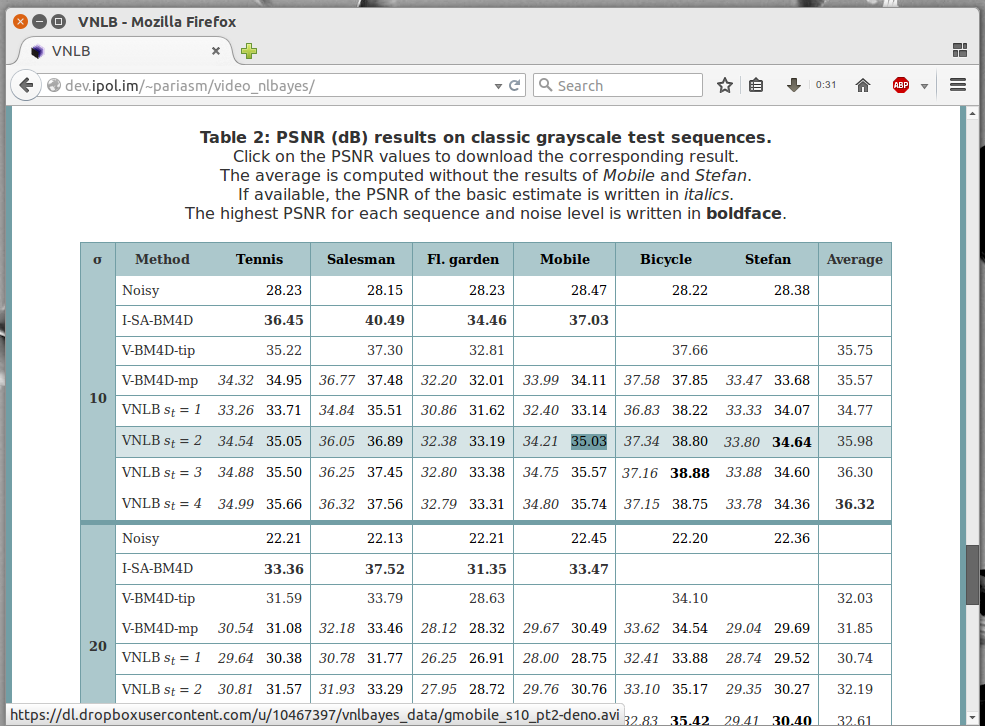
\includegraphics[width=.8\textwidth]{vnlb_web.png}
	\end{center}
\end{frame}


%-cambridge results-% \begin{frame}{PSNRs for grayscale test sequences}
%-cambridge results-% 	\begin{center}
%-cambridge results-% 		{\small
%-cambridge results-% 		\renewcommand{\tabcolsep}{2mm}
%-cambridge results-% 		\renewcommand{\arraystretch}{1.0}
%-cambridge results-% 		\begin{tabular}{ c | l |c c | c c | c c | c c}
%-cambridge results-% 			\hline
%-cambridge results-% 			\rule{0pt}{6pt}$\sigma$ & Method             & \multicolumn{2}{c}{Tennis}  & \multicolumn{2}{c}{Mobile}  &\multicolumn{2}{c}{Stefan}   & \multicolumn{2}{c}{Football} \\\hline
%-cambridge results-% 			\multirow{5}{*}{$10$} & V-BM4D-mp            & \bsic{34.32} &       34.95  & \bsic{33.99} &       34.11  & \bsic{33.47} &       33.68  & \bsic{34.22} &       34.95  \\
%-cambridge results-% %			                      & VNLB   $s_t = 1$     & \bsic{todo } &       todo   & \bsic{todo } &       todo   & \bsic{todo } &       todo   & \bsic{todo } &       todo   \\
%-cambridge results-% 			                      & VNLB   $s_t = 2$     & \bsic{34.33} &       34.62  & \bsic{34.44} &       34.67  & \Bsic{33.82} & \Best{34.23} & \Bsic{34.91} &       35.61  \\
%-cambridge results-% 										 & VNLB   $s_t = 3$     & \Bsic{34.53} &       35.15  & \Bsic{34.74} &       35.31  & \Bsic{33.81} & \Best{34.29} & \bsic{34.70} & \Best{35.67} \\
%-cambridge results-% 			                      & VNLB   $s_t = 4$     & \bsic{34.18} & \Best{35.32} & \bsic{34.41} & \Best{35.54} & \bsic{33.47} &       34.13  & \bsic{34.18} &       35.61  \\\hline
%-cambridge results-% %
%-cambridge results-% 			\multirow{5}{*}{$20$} & V-BM4D-mp            & \bsic{30.54} &       31.08  & \bsic{29.67} &       30.49  & \bsic{29.04} &       29.69  & \bsic{30.16} &       31.06  \\
%-cambridge results-% %			                      & VNLB   $s_t = 1$     & \bsic{todo } &       todo   & \bsic{todo } &       todo   & \bsic{todo } &       todo   & \bsic{todo } &       todo   \\
%-cambridge results-% 			                      & VNLB   $s_t = 2$     & \Bsic{30.73} &       31.24  & \bsic{29.83} &       30.34  & \Bsic{29.38} &       29.90  & \Bsic{30.96} & \Best{31.82} \\
%-cambridge results-% 										 & VNLB   $s_t = 3$     & \Bsic{30.82} &       31.66  & \Bsic{30.15} &       31.09  & \Bsic{29.33} & \Best{30.02} & \bsic{30.67} & \Best{31.83} \\
%-cambridge results-% 			                      & VNLB   $s_t = 4$     & \bsic{30.25} & \Best{31.69} & \bsic{29.74} & \Best{31.35} & \bsic{28.89} & \Best{29.97} & \bsic{29.96} &       31.66  \\\hline
%-cambridge results-% %
%-cambridge results-% 			\multirow{5}{*}{$40$} & V-BM4D-mp            & \bsic{27.67} &       28.38  & \bsic{24.64} &       26.02  & \bsic{24.47} &       25.64  & \bsic{26.67} &       27.62  \\
%-cambridge results-% %			                      & VNLB   $s_t = 1$     & \bsic{todo } &       todo   & \bsic{todo } &       todo   & \bsic{todo } &       todo   & \bsic{todo } &       todo   \\
%-cambridge results-% 			                      & VNLB   $s_t = 2$     & \bsic{27.14} &       28.15  & \bsic{25.43} &       26.06  & \bsic{25.18} &       25.81  & \bsic{27.23} &       28.24  \\
%-cambridge results-% 										 & VNLB   $s_t = 3$     & \bsic{27.63} &       28.62  & \bsic{26.15} &       26.94  & \Bsic{25.44} & \Best{26.12} & \Bsic{27.37} & \Best{28.42} \\
%-cambridge results-% 			                      & VNLB   $s_t = 4$     & \Bsic{27.81} & \Best{28.86} & \Bsic{26.45} & \Best{27.46} & \Bsic{25.50} & \Best{26.24} & \Bsic{27.31} & \Best{28.45} \\\hline
%-cambridge results-% 		\end{tabular}}
%-cambridge results-% % Command to print rounded psnrs
%-cambridge results-% % for i in $(cat bus_s40_pt*/measures | grep PSNR_final | sed "s/^-PSNR_final\ =\ "//); do  echo "scale=2;(((10^2)*$i)+0.5)/(10^2)" | bc; done
%-cambridge results-% 
%-cambridge results-% 		\bigskip
%-cambridge results-% 
%-cambridge results-% 		PSNRs obtained for the four classic color test sequences.
%-cambridge results-% 	\end{center}
%-cambridge results-% \end{frame}




\section{Detailed description of VNLB}

\begin{frame}{A Gaussian linear model for patches}

	\structure{Observation model:} We assume additive white Gaussian noise (AGWN):
	\[v = u + n,\]
	where $u,v,n:\Omega\times \{1,\cdots,T\}\rightarrow\mathds R$ and $n(x,t)\sim \mathcal N(0,\sigma^2)$.

	\bigskip                        

	\pause

	\structure{\emph{A priori} model for 3D patches:} Let $\ma p_{xt}$ be a
	$s_x\times s_x\times s_t$ patch from $u$ located at $(x,t)$. 
%	In a locality of $\ma p_{xt}$, 
%	the set of 3D patches from $u$ are assumed to follow a Gaussian distribution. 
	We assume that $\ma p_{xt}$ follows a Gaussian distribution.


%	\begin{equation*}
%		\mathds{P}(\ma p) = \mathcal N(\overline {\ma p}, C_{\ma p}) \propto \exp\left(-\frac12\langle \ma p - \overline{\ma p}, C_{\ma p}^{-1}(\ma p - \overline{\ma p})\rangle\right)
%	\end{equation*}

	\bigskip

	\pause

	\begin{block}{Local Gaussian model for 3D patches}
	Alltogether, we have the following local model for 3D patches:
	\begin{align*}
		\mathds{P}(\ma p_{xt}) &= \mathcal N(\ma p_{xt}\,|\,\overline {\ma p}_{xt}, C_{xt}) 
		                   \propto \exp\left(-\frac12\langle \ma p_{xt} - \overline{\ma p}_{xt}, 
		                                C_{xt}^{-1}(\ma p_{xt} - \overline{\ma p}_{xt})\rangle\right)\\
		\mathds{P}(\ma q_{xt}|\ma p_{xt}) &= \mathcal N(\ma q_{xt}\,|\,\ma p_{xt}, \sigma^2 I) 
		             \propto \exp\left(-\frac1{2\sigma^2}\|\ma q_{xt} - \ma p_{xt}\|^2\right)
	\end{align*}
	Where 
%	\begin{equation*}
	$
		\quad \ma p_{xt}  \,\, \text{is a patch from } u \text{ and }
		\quad \ma q_{xt}  \,\, \text{is the corresponding patch from } v.
	$
%	\end{equation*}
	\end{block}

\end{frame}

\begin{frame}{Patch denoising via MAP inference}

	Assume for now that we know $\overline{\ma p}$ and $C$.

	\bigskip

	Given a noisy patch $\ma q$, we estimate its noiseless version 
	as the \emph{maximum a posteriori} (MAP):
	\begin{align*}
		\widetilde{\ma p} &:= \argmax_{\ma p} \mathds P(\ma p | \ma q) 
								 = \argmin_{\ma p} -\log \mathds P(\ma p | \ma q)\\
								&\,\,= \overline{\ma p} + C(C
								 + \sigma^2 I)^{-1}(\ma q - \overline{\ma p})
	\end{align*}

	\bigskip

	\pause

	If $C = U\Lambda U^T$ is the eigendecomposition of $C$, we have that
	\[U^T(\widetilde{\ma p} - \overline{\ma p}) \,\,\,\, = \,\,\,\, 
		\Lambda(\Lambda + \sigma^2 I)^{-1}\,\,\,\,
		U^T (\ma q - \overline{\ma p})\]

	\bigskip

	\pause

	\[W = \Lambda(\Lambda + \sigma^2I)^{-1}\quad\rightarrow \quad 
		w_{ii} = \frac{\lambda_i}{\lambda_i + \sigma^2}
	%	       = (1 + \sigma^2/\lambda_i)^{-1}
				 = (1 + \text{snr}_i^{-1})^{-1}\]

	\begin{center}
		\begin{tabular}[c]{c p{7cm} c}
		\structure{$\ma \Longrightarrow$} &
		\centering Diagonal operator in the basis of principal directions: \\ 
		\structure{Wiener filter on the principal components of $\ma q$.} &
		\structure{$\ma \Longleftarrow$}
		\end{tabular}
	\end{center}

\end{frame}

\begin{frame}{Learning the local Gaussian models}

	Marginal distribution for noisy patches:
	$\mathds{P}(\ma q) = \mathcal{N}(\ma q \,|\,\overline{\ma p}, C + \sigma^2I).$

	\bigskip

	\bigskip

	\bigskip

	Given a set of patches $\ma q_i \sim \mathcal{N}(\ma q \,|\,\overline{\ma
	p}, C + \sigma^2I)$, $i = 1,\dots,n$, we have the following \emph{maximum likelihood} estimates
	of the parameters:

	\begin{equation*}
		\widehat{\overline{\ma p}} = \frac1n\sum_{i = 1}^n \ma q_i
		\quad\quad\text{and}\quad\quad\quad
		\widehat{C} = \frac1n\sum_{i = 1}^n \ma q_i^T\ma q_i - \sigma^2 I
	\end{equation*}

	\bigskip

	\bigskip

	\bigskip

	In practice, for a noisy patch $\ma q$, we look for its $n_{\text{sim}}$
	nearest neighbors and assume that they are samples from a single Gaussian
	model. 

\end{frame}

\begin{frame}{Additional assumption: low dimensional patch manifold}

	\structure{Assumption:} Locally, the set of noiseless patches
	can be approximated by a hyperplane of dimension $r$.

	\bigskip

	\structure{Linear Gaussian model:} This translates into a rank $r$
	covariance matrix: \[C = WW^T, \quad\quad\text{with }W \text{ a }d\times r \text{ full rank matrix}.\] 

	\bigskip

	\structure{ML learning:} The \emph{maximum likelihood} estimate of $C$ is then 
	\[\widehat{C}_r = \widehat{U}_r\widehat{\Lambda}_r\widehat{U}^T_r\]
	where $\widehat{U}_r$, $d\times r$ and $\widehat{\Lambda}_r =
	\text{diag}(\lambda_1, \lambda_2,\dots,\lambda_r)$ are the largest 
	$r$ eigenvectors and eigenvalues of $\widehat{C}$.

	\bigskip

	\structure{MAP inference:} Same as before, but can be computed more
	efficiently.


\end{frame}


\begin{frame}{Examples of local Gaussian models}
	\centering
	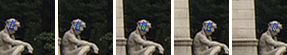
\includegraphics[width = \textwidth]{figs/patch_groups/patch_group_bus_045_085_012_s40_wx37_wt2_sx9_st4_r040_n200_coor.png}\\
	\vspace{.2cm}
	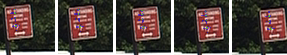
\includegraphics[width = \textwidth]{figs/patch_groups/patch_group_bus_255_056_010_s40_wx37_wt2_sx9_st4_r040_n200_coor.png}
%	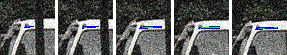
\includegraphics[width = \textwidth]{figs/patch_groups/patch_group_bus_110_090_010_s40_wx37_wt2_sx9_st4_r040_n200_coor.png}

	\bigskip

	Groups of 200 similar $9\times 9\times 4$ patches, in a $37\times37\times5$ search region. 

	\bigskip

	\textcolor{red}{Nearest neighbors 1 to 5.}

	\textcolor{green}{Nearest neighbors 6 to 45.}

	\textcolor{blue}{Nearest neighbors 46 to 200.}

%	In red we show the positions of the 5 nearest neighbors, in green the next 40 and in blue the rest.
%	Note the points shown correspond to the top-left pixel of the first spatial
%	slice of each patch.
%	The reference patch is the red patch in the center of the search region. To highlight the
%	position of the patches, the color of the images has been attenuated.
\end{frame}

\begin{frame}{Examples of local Gaussian models}
%-large screens-%	\begin{center}
%-large screens-%%	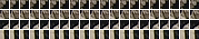
\includegraphics[width = .495\columnwidth]{figs/patch_groups/patch_group_bus_045_085_012_s40_wx37_wt2_sx9_st4_r040_n200_orig.png}\\
%-large screens-%%	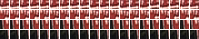
\includegraphics[width = .495\columnwidth]{figs/patch_groups/patch_group_bus_255_056_010_s40_wx37_wt2_sx9_st4_r040_n200_orig.png}\\
%-large screens-%%	\vspace{.1cm}
%-large screens-%	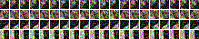
\includegraphics[width = .495\columnwidth]{figs/patch_groups/patch_group_bus_045_085_012_s40_wx37_wt2_sx9_st4_r040_n200_nisy.png} \hfill
%-large screens-%	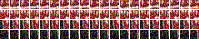
\includegraphics[width = .495\columnwidth]{figs/patch_groups/patch_group_bus_255_056_010_s40_wx37_wt2_sx9_st4_r040_n200_nisy.png}\\
%-large screens-%	\vspace{.1cm}
%-large screens-%	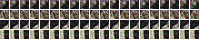
\includegraphics[width = .495\columnwidth]{figs/patch_groups/patch_group_bus_045_085_012_s40_wx37_wt2_sx9_st4_r040_n200_deno.png} \hfill
%-large screens-%	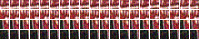
\includegraphics[width = .495\columnwidth]{figs/patch_groups/patch_group_bus_255_056_010_s40_wx37_wt2_sx9_st4_r040_n200_deno.png}\\
%-large screens-%	\vspace{.1cm}
%-large screens-%	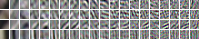
\includegraphics[width = .495\columnwidth]{figs/patch_groups/patch_group_bus_045_085_012_s40_wx37_wt2_sx9_st4_r040_n200_pcas.png} \hfill
%-large screens-%	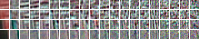
\includegraphics[width = .495\columnwidth]{figs/patch_groups/patch_group_bus_255_056_010_s40_wx37_wt2_sx9_st4_r040_n200_pcas.png}\\
%-large screens-%%	\vspace{.1cm}
%-large screens-%	\end{center}

	\begin{center}
%	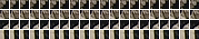
\includegraphics[width = .495\columnwidth]{figs/patch_groups/patch_group_bus_045_085_012_s40_wx37_wt2_sx9_st4_r040_n200_orig.png}\\
%	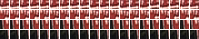
\includegraphics[width = .495\columnwidth]{figs/patch_groups/patch_group_bus_255_056_010_s40_wx37_wt2_sx9_st4_r040_n200_orig.png}\\
%	\vspace{.2cm}
	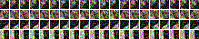
\includegraphics[width = .8\columnwidth]{figs/patch_groups/patch_group_bus_045_085_012_s40_wx37_wt2_sx9_st4_r040_n200_nisy.png}\\
%	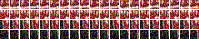
\includegraphics[width = .495\columnwidth]{figs/patch_groups/patch_group_bus_255_056_010_s40_wx37_wt2_sx9_st4_r040_n200_nisy.png}\\
	\vspace{.2cm}
	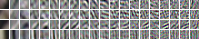
\includegraphics[width = .8\columnwidth]{figs/patch_groups/patch_group_bus_045_085_012_s40_wx37_wt2_sx9_st4_r040_n200_pcas.png}\\
%	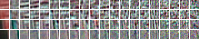
\includegraphics[width = .495\columnwidth]{figs/patch_groups/patch_group_bus_255_056_010_s40_wx37_wt2_sx9_st4_r040_n200_pcas.png}\\
	\vspace{.2cm}
	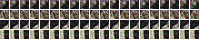
\includegraphics[width = .8\columnwidth]{figs/patch_groups/patch_group_bus_045_085_012_s40_wx37_wt2_sx9_st4_r040_n200_deno.png}\\
%	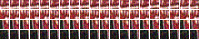
\includegraphics[width = .495\columnwidth]{figs/patch_groups/patch_group_bus_255_056_010_s40_wx37_wt2_sx9_st4_r040_n200_deno.png}\\
%	\vspace{.1cm}
	\end{center}

	\medskip

	\begin{description}
		\item[Top:] 20 nearest neighbors (noisy).

		\item[Center:] sample mean and first 19 principal directions.

		\item[Bottom:] corresponding MAP estimates.
	\end{description}

	%Each column corresponds to the 4 spatial slices of a $9\times9\times4$ patch.
\end{frame}

%\begin{frame}
%	\centering
%%	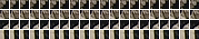
\includegraphics[width = .45\columnwidth]{figs/patch_groups/patch_group_bus_045_085_012_s40_wx37_wt2_sx9_st4_r040_n200_orig.png}\\
%%	\vspace{.1cm}
%%	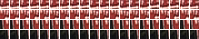
\includegraphics[width = .45\columnwidth]{figs/patch_groups/patch_group_bus_255_056_010_s40_wx37_wt2_sx9_st4_r040_n200_orig.png}\\
%%	\vspace{.1cm}
%%	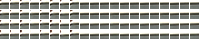
\includegraphics[width = .45\columnwidth]{figs/patch_groups/patch_group_bus_110_090_010_s40_wx37_wt2_sx9_st4_r040_n200_orig.png}\\
%%	\vspace{.1cm}
%	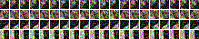
\includegraphics[width = .45\columnwidth]{figs/patch_groups/patch_group_bus_045_085_012_s40_wx37_wt2_sx9_st4_r040_n200_nisy.png}\\
%	\vspace{.2cm}
%	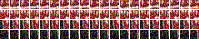
\includegraphics[width = .45\columnwidth]{figs/patch_groups/patch_group_bus_255_056_010_s40_wx37_wt2_sx9_st4_r040_n200_nisy.png}\\
%	\vspace{.2cm}
%%	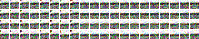
\includegraphics[width = .45\columnwidth]{figs/patch_groups/patch_group_bus_110_090_010_s40_wx37_wt2_sx9_st4_r040_n200_nisy.png}\\
%%	\vspace{.1cm}
%	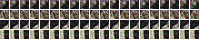
\includegraphics[width = .45\columnwidth]{figs/patch_groups/patch_group_bus_045_085_012_s40_wx37_wt2_sx9_st4_r040_n200_deno.png}\\
%	\vspace{.2cm}
%	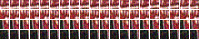
\includegraphics[width = .45\columnwidth]{figs/patch_groups/patch_group_bus_255_056_010_s40_wx37_wt2_sx9_st4_r040_n200_deno.png}\\
%	\vspace{.2cm}
%%	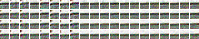
\includegraphics[width = .45\columnwidth]{figs/patch_groups/patch_group_bus_110_090_010_s40_wx37_wt2_sx9_st4_r040_n200_deno.png}\\
%%	\vspace{.1cm}
%	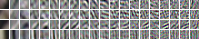
\includegraphics[width = .45\columnwidth]{figs/patch_groups/patch_group_bus_045_085_012_s40_wx37_wt2_sx9_st4_r040_n200_pcas.png}\\
%	\vspace{.2cm}
%	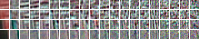
\includegraphics[width = .45\columnwidth]{figs/patch_groups/patch_group_bus_255_056_010_s40_wx37_wt2_sx9_st4_r040_n200_pcas.png}\\
%	\vspace{.2cm}
%%	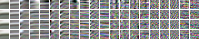
\includegraphics[width = .45\columnwidth]{figs/patch_groups/patch_group_bus_110_090_010_s40_wx37_wt2_sx9_st4_r040_n200_pcas.png}\\
%%	\vspace{.1cm}
%
%	\bigskip
%
%	The 20 nearest neighbors (top), the corresponding MAP estimates (middle) and the sample mean 
%	and first 19 principal directions computed from the sample covariance matrix (bottom).
%	For each image, each column corresponds to the 4 spatial slices of a $9\times9\times4$ patch.
%\end{frame}

\begin{frame}{Algorithm}

%	\caption{Video NL-Bayes}
%	\label{alg:nlbayes}

	\begin{columns}
	\begin{column}{0.8\textwidth}
	\begin{overprint}

		\onslide<1>
		\begin{algorithm}[H]
			\caption{Video NL-Bayes - Step 1: basic estimate}
			\begin{spacing}{1.3}
				\begin{algorithmic}[1]
				\REQUIRE Noisy video $v$, noise std. dev.
				$\sigma$\textcolor{white}{, basic estimate $u^{(1)}$}
				\ENSURE Basic estimate of noiseless video $\widetilde u^{(1)}$
				\STATE Set $\mathcal P = \{\ma q \,:\, \ma q \text{ patch of }  v\}$ \COMMENT{patches to process}
				\WHILE{$\mathcal P \neq \emptyset$}
				\STATE Get a patch $\ma q$ from $\mathcal P$ \COMMENT{``center'' of Gaussian model}
					\STATE Retrieve $n_{\text{sim}}$ nearest neighbors of $\ma
					q$ in spatio-temporal volume around $\ma q$.\textcolor{white}{ The
						distance is computed using basic estimates
						$\widetilde{\ma p}^{(1)}$.}
					\STATE Compute $\widehat{\overline{\ma p}}\,\!^{(1)}$, 
					$\widehat C_{r}^{(1)}$ \textcolor{white}{from basic
						estimates $\widetilde{\ma p}_i^{(1)}$, \textbf{setting} $\ma{\sigma = 0}$.}
					\FORALL{$n_{\text{sim}}$ neighbors $\ma q_i$ of $\ma q$}
						\STATE Obtain the MAP estimate $\widetilde{\ma p}_i^{(1)}$
						\STATE Aggregate estimated patch on $\widetilde u^{(1)}$
						\STATE Remove $\ma q_i$ from $\mathcal P$
					\ENDFOR
				\ENDWHILE
	%			\FORALL{pixel $(x,t)$ in $\Omega\times {1,\dots,T}$}
	%			\STATE Obtain the basic estimate $\widetilde u^{(1)}(x,t)$ by averaging
	%			the values of all patches $\widetilde{\ma p}^{(1)}$ containing $(x,t)$.
	%			\ENDFOR
			\end{algorithmic}
			\end{spacing}
		\end{algorithm}

		\onslide<2>
		\begin{algorithm}[H]
		\caption{Video NL-Bayes - Step 2: final estimate}
			\begin{spacing}{1.3}
				\begin{algorithmic}[1]
				\REQUIRE Noisy video $v$, noise std. dev.
				$\sigma$, \structure{basic estimate $\widetilde u^{(1)}$} 
				\ENSURE Final estimate of noiseless video $\widetilde u^{(2)}$
				\STATE Set $\mathcal P = \{\ma q \,:\, \ma q \text{ patch of }  v\}$ \COMMENT{patches to process}
				\WHILE{$\mathcal P \neq \emptyset$}
				\STATE Get a patch $\ma q$ from $\mathcal P$ \COMMENT{``center'' of Gaussian model}
					\STATE Retrieve $n_{\text{sim}}$ nearest neighbors of $\ma
					q$ in spatio-temporal volume around $\ma q$.
					\structure{The distance is computed using basic estimates
						$\widetilde{\ma p}^{(1)}$.}
					\STATE Compute $\widehat{\overline{\ma p}}\,\!^{(2)}$, $\widehat
							 C_{r}^{(2)}$ \structure{from basic estimates
								 $\widetilde{\ma p}_i^{(1)}$, \textbf{setting} $\ma{\sigma = 0}$.}
					\FORALL{$n_{\text{sim}}$ neighbors $\ma q_i$ of $\ma q$}
						\STATE Obtain the MAP estimate $\widetilde{\ma p}_i^{(2)}$
						\STATE Aggregate estimated patch on $\widetilde u^{(2)}$
						\STATE Remove $\ma q_i$ from $\mathcal P$
					\ENDFOR
				\ENDWHILE
	%			\FORALL{pixel $(x,t)$ in $\Omega\times {1,\dots,T}$}
	%			\STATE Obtain the basic estimate $\widetilde u^{(1)}(x,t)$ by averaging
	%			the values of all patches $\widetilde{\ma p}^{(1)}$ containing $(x,t)$.
	%			\ENDFOR
			\end{algorithmic}
			\end{spacing}
		\end{algorithm}

	\end{overprint}
	\end{column}%
%	\begin{column}{0.4\textwidth}
%	\end{column}
	\end{columns}

	\vspace{1cm}

\end{frame}

% \begin{frame}{Note: learning in 2nd stage}
% 
% 	In the second stage the basic estimate is used as an oracle to estimate
% 	patch distances and to learn the parameters of the Gaussian linear models.
% 
% 	\bigskip
% 
% 	Since the set of patches from the basic estimate $\ma p^{(1)}_i$ are considered to
% 	be noiseless, the maximum likelihood parameters are as follows:
% 
% 	\begin{equation*}
% 		\widehat{\overline{\ma p}}\,\!^{(2)} = \frac1n\sum_{i = 1}^n \ma p^{(1)}_i
% 		\quad\quad\text{and}\quad\quad\quad
% 		\widehat{C}^{(2)} = \frac1n\sum_{i = 1}^n \ma p^{(1)\,T}_i\ma p^{(1)}_i
% 	\end{equation*}
% 	
% \end{frame}


\begin{frame}{Color videos}

	We follow \reference{Lebrun et al.'13, Dabov et al.'07}.

	\bigskip

	\setbeamertemplate{itemize items}[triangle]
	
	In the first stage: 
	\begin{itemize}\itemsep=.3cm
		\item Use YUV colorspace (opponent color transform).
		\item Patch distance computed using luminance Y only.
		\item A Gaussian model is learnt for each channel (i.e. zero covariances
			between channels)
	\end{itemize}

	\bigskip

	\bigskip

	In the second stage: 
	\begin{itemize}\itemsep=.3cm
		\item Patch distance computed using the three RGB color channels.
		\item A Gaussian model is learnt jointly for the RGB patches.
	\end{itemize}
	
\end{frame}

% \begin{frame}{Results}
% 
% 	\begin{center}
% 	Experiments on 5 sequences of the Middlebury optical flow dataset:
% 
% 	\bigskip
% 
% 	\emph{Army}, \\
% 	\emph{DogDance}, \\
% 	\emph{Evergreen}, \\
% 	\emph{Mequon}, \\
% 	\emph{Walking},
% 
% 	\bigskip
% 
% 	with white additive Gaussian noise of 
% 
% 	\bigskip
% 	
% 	$\sigma = 10$, \\ 
% 	$\sigma = 20$, \\ 
% 	$\sigma = 40$.
% 	\end{center}
% 
% \end{frame}



% % \begin{frame}{Comparison with V-BM4D}
% % 
% % 	We compare with V-BM4D \reference{Maggioni et al.'12}.
% % 
% % 	\setbeamertemplate{itemize items}[triangle]
% % 
% % 	\begin{itemize}\itemsep=.3cm
% % 		\item Two stages comprised of \emph{building of patch trajectories}, \emph{grouping}, \emph{collaborative
% % 			filtering}, and \emph{aggregation}.
% % 		\item \structure{Patch trajectories} built using block matching.
% % 		\item \structure{Grouping:} for each spatio-temporal patch $\ma q_0$, a
% % 			group of similar patches is build as
% % 			\[\mathcal G(\ma q_0) = \{\ma  q \text{ spatio-temporal patch}\,:\, d(\ma q_0, \ma q) < \tau_{\text{match}}\}\]
% % 		\item \structure{Collaborative filtering:} Each group $\mathcal G(\ma q)$ of similar 3D
% % 			patches is treated as a 4D signal which is filtered in a transform
% % 			domain, via thresholding (1st stage) or Wiener filtering (2nd stage). 
% % 	\end{itemize}
% % 
% % \end{frame}



\begin{frame}{Parameters}
	\begin{center}

	\begin{tabular}{l | c c | c c | c c }
		& \multicolumn{2}{c|}{$\sigma = 10$} 
		& \multicolumn{2}{c|}{$\sigma = 20$} 
		& \multicolumn{2}{c}{$\sigma = 40$} \\
		                            & 1st    & 2nd   & 1st   & 2nd   & 1st   & 2nd    \\\hline\hline
		Patch size (spatial)        &  7 / 5 & 7 / 5 & ''  & ''  & ''  &  ''  \\
		Patch size (temporal)       &  1--4  & 1--4  & ''  & ''  & ''  &  ''  \\
		Spatial search window       & 45 / 37&45 / 37& ''  & ''  & ''  &  ''  \\
		Temporal search range       & 5      & 5     & ''  & ''  & ''  &  ''  \\
		Number of patches           & 400    & 100   & ''  & ''  & ''  &  ''  \\
		Rank                        & full   & 35    & ''  & 30    & ''  & 20     \\
%		Distance threshold $\tau$   & n/a    & 432   & n/a   & 432   & n/a   & 432    \\
%		Beta                        & 1      & 1.2   & 1     & 1.2   & 1     & 1.2    \\\hline
	\end{tabular}

	\bigskip

	We write \emph{grayscale-parameters / color-parameter} in case\\ a parameter
	differs between grascale and color videos.

%-parameters v-bm4d-%	\pause
%-parameters v-bm4d-%	\bigskip
%-parameters v-bm4d-%
%-parameters v-bm4d-%	\begin{tabular}{l | c c}
%-parameters v-bm4d-%		                              & 1st & 2nd  \\\hline\hline
%-parameters v-bm4d-%		Patch size (spatial)          &  8  &   8  \\
%-parameters v-bm4d-%		Patch size (temporal)         & 15  &  15  \\
%-parameters v-bm4d-%		Spatial search window         & 15  &  15  \\
%-parameters v-bm4d-%		Temporal search range         &  1  &   1  \\
%-parameters v-bm4d-%		Number of patches             & 32  &  32  \\
%-parameters v-bm4d-%		Spatial search window (M.E.)  & 11  &  11  \\
%-parameters v-bm4d-%	\end{tabular}
%-parameters v-bm4d-%
%-parameters v-bm4d-%	\vspace{.1cm}
%-parameters v-bm4d-%	Parameters of V-BM4D (M.E.: motion estimation)
%-parameters v-bm4d-%
	\end{center}
\end{frame}




%-temporal consistency-% \begin{frame}{Temporal consistency of the result}
%-temporal consistency-% 	\begin{center}
%-temporal consistency-% 		\includegraphics<1>[width=.9\textwidth]{figures/bus_slice100_s40.png}
%-temporal consistency-% 		\includegraphics<2>[width=.9\textwidth]{figures/bus_slice100_s40_vbm4d.png}
%-temporal consistency-% 		\includegraphics<3>[width=.9\textwidth]{figures/bus_slice100_s40_vnlb3d.png}
%-temporal consistency-% 		\includegraphics<4>[width=.9\textwidth]{figures/bus_slice100.png}
%-temporal consistency-% 	%	\includegraphics<2>[width=.7\textwidth]{figures/bus_slice100_s10.png}
%-temporal consistency-% 	%	\includegraphics<3>[width=.7\textwidth]{figures/bus_slice100_s10_vbm4d.png}
%-temporal consistency-% 	%	\includegraphics<4>[width=.7\textwidth]{figures/bus_slice100_s10_vnlb3d.png}
%-temporal consistency-% 	%	\includegraphics<5>[width=.7\textwidth]{figures/bus_slice100_s20.png}
%-temporal consistency-% 	%	\includegraphics<6>[width=.7\textwidth]{figures/bus_slice100_s20_vbm4d.png}
%-temporal consistency-% 	%	\includegraphics<7>[width=.7\textwidth]{figures/bus_slice100_s20_vnlb3d.png}
%-temporal consistency-% 	\end{center}
%-temporal consistency-% 
%-temporal consistency-% 	\bigskip
%-temporal consistency-% 
%-temporal consistency-% 	\bigskip
%-temporal consistency-% 
%-temporal consistency-% 	\centerline{Horizontal slice of a video. Each row corresponds to a different frame.}
%-temporal consistency-% 		\begin{overprint}
%-temporal consistency-% 			\onslide<1> \centerline{Original video contaminted with AWGN of $\sigma = 40$.}
%-temporal consistency-% 			\onslide<2> \centerline{Result of V-BM4D-mp.}
%-temporal consistency-% 			\onslide<3> \centerline{Result of VNLB.}
%-temporal consistency-% 			\onslide<4> \centerline{Original video.}
%-temporal consistency-% 		\end{overprint}
%-temporal consistency-% 		
%-temporal consistency-% \end{frame}



%-challenging cases-% \multipleframe
%-challenging cases-% % stefan detail1 
%-challenging cases-% \begin{frame}{Example of a challenging sequence}
%-challenging cases-% 	\begin{center}
%-challenging cases-% % 			\animategraphics[palindrome, controls, autopause, height=4cm]{2}{VBM4D/stefan_mono_mp_s20/tile090-180-265_}{001}{010}
%-challenging cases-% % 			\animategraphics[palindrome, controls, autopause, height=4cm]{2}{vnlb3d_mono/stefan_mono_s20_pt4/tile090-180-265_}{001}{010}
%-challenging cases-% 			\begin{animateinline}[palindrome, autoplay]{10}
%-challenging cases-% 				\multiframe{30}{i=1+1}{%
%-challenging cases-% 				\begin{tabular}{c}
%-challenging cases-% 					\includegraphics[height=3.5cm]{data/derf/stefan_mono/tile090-180-265_\zeropad{123}{\i}}$\,$ 
%-challenging cases-% 					\includegraphics[height=3.5cm]{vnlb3d_mono/stefan_mono_s10_pt4/nisy_tile090-180-265_\zeropad{123}{\i}}\\
%-challenging cases-% 					\includegraphics[height=3.5cm]{VBM4D/stefan_mono_mp_s10/tile090-180-265_\zeropad{123}{\i}}$\,$ 
%-challenging cases-% 					\includegraphics[height=3.5cm]{vnlb3d_mono/stefan_mono_s10_pt4/tile090-180-265_\zeropad{123}{\i}}
%-challenging cases-% 				\end{tabular}
%-challenging cases-% 				}
%-challenging cases-% 			\end{animateinline}
%-challenging cases-% 	\end{center}
%-challenging cases-% 
%-challenging cases-% 	\begin{center}
%-challenging cases-% 		\emph{Stefan} (detail). Top: original and noisy ($\sigma = 10$), bottom: V-BM4D-mp and VNLB.
%-challenging cases-% 	\end{center}
%-challenging cases-% \end{frame}
%-challenging cases-% \begin{frame}{Example of a challenging sequence}
%-challenging cases-% 	\begin{center}
%-challenging cases-% % 			\animategraphics[palindrome, controls, autopause, height=4cm]{2}{VBM4D/stefan_mono_mp_s20/tile090-180-265_}{001}{010}
%-challenging cases-% % 			\animategraphics[palindrome, controls, autopause, height=4cm]{2}{vnlb3d_mono/stefan_mono_s20_pt4/tile090-180-265_}{001}{010}
%-challenging cases-% 			\begin{animateinline}[palindrome, autoplay]{10}
%-challenging cases-% 				\multiframe{30}{i=1+1}{%
%-challenging cases-% 				\begin{tabular}{c}
%-challenging cases-% 					\includegraphics[height=3.5cm]{data/derf/stefan_mono/tile090-180-265_\zeropad{123}{\i}}$\,$ 
%-challenging cases-% 					\includegraphics[height=3.5cm]{vnlb3d_mono/stefan_mono_s20_pt4/nisy_tile090-180-265_\zeropad{123}{\i}}\\
%-challenging cases-% 					\includegraphics[height=3.5cm]{VBM4D/stefan_mono_mp_s20/tile090-180-265_\zeropad{123}{\i}}$\,$ 
%-challenging cases-% 					\includegraphics[height=3.5cm]{vnlb3d_mono/stefan_mono_s20_pt4/tile090-180-265_\zeropad{123}{\i}}
%-challenging cases-% 				\end{tabular}
%-challenging cases-% 				}
%-challenging cases-% 			\end{animateinline}
%-challenging cases-% 	\end{center}
%-challenging cases-% 
%-challenging cases-% 	\begin{center}
%-challenging cases-% 		\emph{Stefan} (detail). Top: original and noisy ($\sigma = 20$), bottom: V-BM4D-mp and VNLB.
%-challenging cases-% 	\end{center}
%-challenging cases-% \end{frame}
%-challenging cases-% \begin{frame}{Example of a challenging sequence}
%-challenging cases-% 	\begin{center}
%-challenging cases-% % 			\animategraphics[palindrome, controls, autopause, height=4cm]{2}{VBM4D/stefan_mono_mp_s20/tile090-180-265_}{001}{010}
%-challenging cases-% % 			\animategraphics[palindrome, controls, autopause, height=4cm]{2}{vnlb3d_mono/stefan_mono_s20_pt4/tile090-180-265_}{001}{010}
%-challenging cases-% 			\begin{animateinline}[palindrome, autoplay]{10}
%-challenging cases-% 				\multiframe{30}{i=1+1}{%
%-challenging cases-% 				\begin{tabular}{c}
%-challenging cases-% 					\includegraphics[height=3.5cm]{data/derf/stefan_mono/tile090-180-265_\zeropad{123}{\i}}$\,$ 
%-challenging cases-% 					\includegraphics[height=3.5cm]{vnlb3d_mono/stefan_mono_s40_pt4/nisy_tile090-180-265_\zeropad{123}{\i}}\\
%-challenging cases-% 					\includegraphics[height=3.5cm]{VBM4D/stefan_mono_mp_s40/tile090-180-265_\zeropad{123}{\i}}$\,$ 
%-challenging cases-% 					\includegraphics[height=3.5cm]{vnlb3d_mono/stefan_mono_s40_pt4/tile090-180-265_\zeropad{123}{\i}}
%-challenging cases-% 				\end{tabular}
%-challenging cases-% 				}
%-challenging cases-% 			\end{animateinline}
%-challenging cases-% 	\end{center}
%-challenging cases-% 
%-challenging cases-% 	\begin{center}
%-challenging cases-% 		\emph{Stefan} (detail). Top: original and noisy ($\sigma = 40$), bottom: V-BM4D-mp and VNLB.
%-challenging cases-% 	\end{center}
%-challenging cases-% \end{frame}
%-challenging cases-% \restoreframe
%-challenging cases-% 
%-challenging cases-% % stefan detail2 
%-challenging cases-% \multipleframe
%-challenging cases-% \begin{frame}{Example of a challenging sequence}
%-challenging cases-% 	\begin{center}
%-challenging cases-% % 			\animategraphics[palindrome, controls, autopause, height=4cm]{2}{VBM4D/stefan_mono_mp_s20/tile090-180-265_}{001}{010}
%-challenging cases-% % 			\animategraphics[palindrome, controls, autopause, height=4cm]{2}{vnlb3d_mono/stefan_mono_s20_pt4/tile090-180-265_}{001}{010}
%-challenging cases-% 			\begin{animateinline}[palindrome, autoplay]{10}
%-challenging cases-% 				\multiframe{30}{i=1+1}{%
%-challenging cases-% 				\begin{tabular}{c}
%-challenging cases-% 					\includegraphics[height=3.5cm]{data/derf/stefan_mono/tile060-130-005_\zeropad{123}{\i}}$\,$ 
%-challenging cases-% 					\includegraphics[height=3.5cm]{vnlb3d_mono/stefan_mono_s10_pt4/nisy_tile060-130-005_\zeropad{123}{\i}}\\
%-challenging cases-% 					\includegraphics[height=3.5cm]{VBM4D/stefan_mono_mp_s10/tile060-130-005_\zeropad{123}{\i}}$\,$ 
%-challenging cases-% 					\includegraphics[height=3.5cm]{vnlb3d_mono/stefan_mono_s10_pt4/tile060-130-005_\zeropad{123}{\i}}
%-challenging cases-% 				\end{tabular}
%-challenging cases-% 				}
%-challenging cases-% 			\end{animateinline}
%-challenging cases-% 	\end{center}
%-challenging cases-% 
%-challenging cases-% 	\begin{center}
%-challenging cases-% 		\emph{Stefan} (detail). Top: original and noisy ($\sigma = 10$), bottom: V-BM4D-mp and VNLB.
%-challenging cases-% 	\end{center}
%-challenging cases-% \end{frame}
%-challenging cases-% \begin{frame}{Example of a challenging sequence}
%-challenging cases-% 	\begin{center}
%-challenging cases-% % 			\animategraphics[palindrome, controls, autopause, height=4cm]{2}{VBM4D/stefan_mono_mp_s20/tile090-180-265_}{001}{010}
%-challenging cases-% % 			\animategraphics[palindrome, controls, autopause, height=4cm]{2}{vnlb3d_mono/stefan_mono_s20_pt4/tile090-180-265_}{001}{010}
%-challenging cases-% 			\begin{animateinline}[palindrome, autoplay]{10}
%-challenging cases-% 				\multiframe{30}{i=1+1}{%
%-challenging cases-% 				\begin{tabular}{c}
%-challenging cases-% 					\includegraphics[height=3.5cm]{data/derf/stefan_mono/tile060-130-005_\zeropad{123}{\i}}$\,$ 
%-challenging cases-% 					\includegraphics[height=3.5cm]{vnlb3d_mono/stefan_mono_s20_pt4/nisy_tile060-130-005_\zeropad{123}{\i}}\\
%-challenging cases-% 					\includegraphics[height=3.5cm]{VBM4D/stefan_mono_mp_s20/tile060-130-005_\zeropad{123}{\i}}$\,$ 
%-challenging cases-% 					\includegraphics[height=3.5cm]{vnlb3d_mono/stefan_mono_s20_pt4/tile060-130-005_\zeropad{123}{\i}}
%-challenging cases-% 				\end{tabular}
%-challenging cases-% 				}
%-challenging cases-% 			\end{animateinline}
%-challenging cases-% 	\end{center}
%-challenging cases-% 
%-challenging cases-% 	\begin{center}
%-challenging cases-% 		\emph{Stefan} (detail). Top: original and noisy ($\sigma = 20$), bottom: V-BM4D-mp and VNLB.
%-challenging cases-% 	\end{center}
%-challenging cases-% \end{frame}
%-challenging cases-% \begin{frame}{Example of a challenging sequence}
%-challenging cases-% 	\begin{center}
%-challenging cases-% % 			\animategraphics[palindrome, controls, autopause, height=4cm]{2}{VBM4D/stefan_mono_mp_s20/tile090-180-265_}{001}{010}
%-challenging cases-% % 			\animategraphics[palindrome, controls, autopause, height=4cm]{2}{vnlb3d_mono/stefan_mono_s20_pt4/tile090-180-265_}{001}{010}
%-challenging cases-% 			\begin{animateinline}[palindrome, autoplay]{10}
%-challenging cases-% 				\multiframe{30}{i=1+1}{%
%-challenging cases-% 				\begin{tabular}{c}
%-challenging cases-% 					\includegraphics[height=3.5cm]{data/derf/stefan_mono/tile060-130-005_\zeropad{123}{\i}}$\,$ 
%-challenging cases-% 					\includegraphics[height=3.5cm]{vnlb3d_mono/stefan_mono_s40_pt4/nisy_tile060-130-005_\zeropad{123}{\i}}\\
%-challenging cases-% 					\includegraphics[height=3.5cm]{VBM4D/stefan_mono_mp_s40/tile060-130-005_\zeropad{123}{\i}}$\,$ 
%-challenging cases-% 					\includegraphics[height=3.5cm]{vnlb3d_mono/stefan_mono_s40_pt4/tile060-130-005_\zeropad{123}{\i}}
%-challenging cases-% 				\end{tabular}
%-challenging cases-% 				}
%-challenging cases-% 			\end{animateinline}
%-challenging cases-% 	\end{center}
%-challenging cases-% 
%-challenging cases-% 	\begin{center}
%-challenging cases-% 		\emph{Stefan} (detail). Top: original and noisy ($\sigma = 40$), bottom: V-BM4D-mp and VNLB.
%-challenging cases-% 	\end{center}
%-challenging cases-% \end{frame}
%-challenging cases-% \restoreframe


% \begin{frame}{Computation time}
% 
% 	Computations performed in \texttt{boucantrin} server, using 8 CPU cores.\\
% 	For CIF (352x288) RGB videos, with $\sigma = 40$: 
% 
% 	\bigskip
% 
% 	\begin{center}
% 	\begin{tabular}{r | c c c c}
% 		$p_t$ & 1 & 2 & 3 & 4 \\
% 		$s/\textnormal{frame}$ & x & 7 & 15 & 30 \\
% 	\end{tabular}
% 	\end{center}
% 
% 	\vspace{2cm}
% 
% 	For example, with $p_t = 4$, it takes 2.5 hours ($\times 8$ cores) for 300 CIF frames!
% 
% \end{frame}
% 
% 

\begin{frame}{Conclusions}

	\setbeamertemplate{itemize items}[triangle]

	\begin{itemize}\itemsep=.5cm
		\item Video denoising by Bayesian filtering of groups of similar spatio-temporal patches.
		\item Temporal consistency without motion estimation.
		\item The proposed model works well on objects with uniform motion.
	%	\item Problems:
	%	\begin{itemize}\itemsep=.4cm
				\item Adherence problem: background texture follows the motion of the foreground object.
				\item Fast changes in motion create artifacts (particularly for
					higher noise levels). 
				\item High computational cost: we are currently searching for stategies to alleviate this.
	%		\end{itemize}
		\item Future work: motion compensated search region, other noise models (structured, signal dependent).
	\end{itemize}


\end{frame}

\begin{frame}

	\centerline{\Huge{\textbf{Thank you}}}

\end{frame}

\end{document}

